\documentclass[12pt,a4paper]{article}

% ── Packages ──────────────────────────────────────────────────────────────────
\usepackage[margin=2.5cm]{geometry}
\usepackage{amsmath,amssymb}
\usepackage{graphicx}
\usepackage{xcolor}
\usepackage{tikz}
\usepackage{pgf-umlsd}
\usepackage{pgfplots}
\pgfplotsset{compat=1.18}
\usetikzlibrary{
  shapes.geometric, shapes.multipart, shapes.symbols,
  arrows.meta, positioning, fit, calc, decorations.pathreplacing,
  backgrounds, patterns, matrix, chains, scopes
}
\usepackage{hyperref}
\hypersetup{colorlinks=true, linkcolor=blue!60!black, urlcolor=blue!60!black}
\usepackage{listings}
\usepackage{booktabs}
\usepackage{enumitem}
\usepackage{caption}
\usepackage{subcaption}
\usepackage{mdframed}
\usepackage{fontawesome5}
\usepackage{setspace}
\usepackage{titlesec}
\usepackage{fancyhdr}
\usepackage{tocloft}

% ── Colours ───────────────────────────────────────────────────────────────────
\definecolor{agentblue}{RGB}{41,128,185}
\definecolor{agentgreen}{RGB}{39,174,96}
\definecolor{agentorange}{RGB}{230,126,34}
\definecolor{agentred}{RGB}{192,57,43}
\definecolor{agentpurple}{RGB}{142,68,173}
\definecolor{agentgray}{RGB}{127,140,141}
\definecolor{lightblue}{RGB}{214,234,248}
\definecolor{lightgreen}{RGB}{212,239,223}
\definecolor{lightyellow}{RGB}{252,243,207}
\definecolor{lightpurple}{RGB}{235,222,240}
\definecolor{lightgray}{RGB}{242,243,244}
\definecolor{codebg}{RGB}{248,249,250}

% ── Code listing style ────────────────────────────────────────────────────────
\lstset{
  backgroundcolor=\color{codebg},
  basicstyle=\ttfamily\small,
  keywordstyle=\color{agentblue}\bfseries,
  commentstyle=\color{agentgray}\itshape,
  stringstyle=\color{agentgreen},
  breaklines=true,
  frame=single,
  framerule=0.4pt,
  rulecolor=\color{agentgray!40},
  numbers=left,
  numberstyle=\tiny\color{agentgray},
  xleftmargin=1.5em,
  framexleftmargin=1.5em
}

% ── Page style ────────────────────────────────────────────────────────────────
\pagestyle{fancy}
\fancyhf{}
\fancyhead[L]{\small\textcolor{agentgray}{Agentic Systems: Theory \& Practice}}
\fancyhead[R]{\small\textcolor{agentgray}{\thepage}}
\fancyfoot[C]{\small\textcolor{agentgray}{Lecture Production Pipeline — Technical Documentation}}
\renewcommand{\headrulewidth}{0.4pt}

% ── Title setup ───────────────────────────────────────────────────────────────
\titleformat{\section}{\Large\bfseries\color{agentblue}}{}{0em}{\thesection\quad}[\titlerule]
\titleformat{\subsection}{\large\bfseries\color{agentblue!80!black}}{}{0em}{\thesubsection\quad}
\titleformat{\subsubsection}{\normalsize\bfseries\color{agentblue!60!black}}{}{0em}{\thesubsubsection\quad}

% ── TikZ node styles ──────────────────────────────────────────────────────────
\tikzset{
  agent/.style={
    rectangle, rounded corners=6pt, minimum width=2.8cm, minimum height=1cm,
    draw=agentblue, fill=lightblue, text centered, font=\small\bfseries,
    text=agentblue!80!black
  },
  tool/.style={
    rectangle, rounded corners=4pt, minimum width=2.4cm, minimum height=0.8cm,
    draw=agentgreen, fill=lightgreen, text centered, font=\small,
    text=agentgreen!70!black
  },
  store/.style={
    cylinder, shape border rotate=90, minimum width=2cm, minimum height=1cm,
    draw=agentorange, fill=lightyellow, text centered, font=\small\bfseries,
    text=agentorange!80!black
  },
  decision/.style={
    diamond, minimum width=2.5cm, minimum height=1cm,
    draw=agentpurple, fill=lightpurple, text centered, font=\scriptsize\bfseries,
    text=agentpurple!80!black, aspect=2
  },
  process/.style={
    rectangle, minimum width=2.8cm, minimum height=0.9cm,
    draw=agentgray, fill=lightgray, text centered, font=\small,
    text=black
  },
  arrow/.style={-{Stealth[length=7pt]}, thick, color=agentgray!80!black},
  arrowblue/.style={-{Stealth[length=7pt]}, thick, color=agentblue},
  arrowgreen/.style={-{Stealth[length=7pt]}, thick, color=agentgreen!70!black},
  arroworange/.style={-{Stealth[length=7pt]}, thick, color=agentorange},
  dasharrow/.style={-{Stealth[length=6pt]}, dashed, thick, color=agentgray!60},
  groupbox/.style={
    rectangle, rounded corners=8pt, dashed, thick,
    inner sep=12pt
  }
}

% ─────────────────────────────────────────────────────────────────────────────
\begin{document}

\begin{titlepage}
  \centering
  \vspace*{2cm}

  {\Huge\bfseries\color{agentblue} Agentic Systems:\\[0.4em]
   \large\color{agentblue!70!black} Theory, Architecture, and\\[0.2em]
   \large\color{agentblue!70!black} A Case Study in Automated Lecture Production}

  \vspace{1.5cm}
  \rule{0.8\textwidth}{1.5pt}
  \vspace{1cm}

  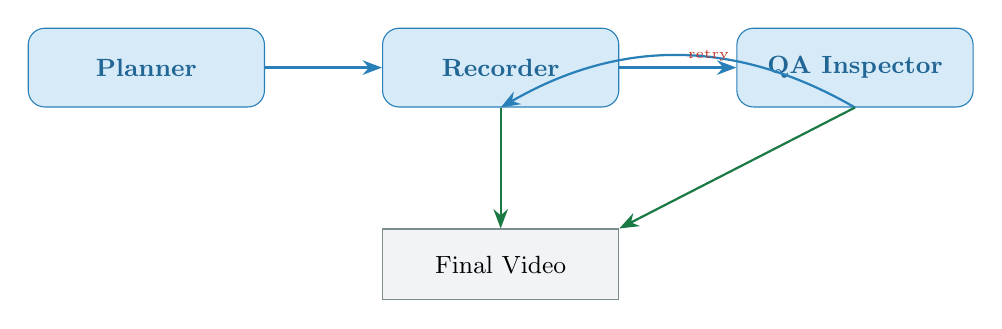
\begin{tikzpicture}
    % Simple visual showing a pipeline
    \node[agent, minimum width=3cm] (plan) at (0,0) {Planner};
    \node[agent, minimum width=3cm] (rec)  at (4.5,0) {Recorder};
    \node[agent, minimum width=3cm] (qa)   at (9,0) {QA Inspector};
    \node[process, minimum width=3cm] (out) at (4.5,-2.5) {Final Video};

    \draw[arrowblue] (plan) -- (rec);
    \draw[arrowblue] (rec)  -- (qa);
    \draw[arrowblue, bend right=30] (qa.south) to node[right, font=\tiny, color=agentred]
      {retry} (rec.south);
    \draw[arrowgreen] (qa.south) -- (out.north east);
    \draw[arrowgreen] (rec.south) -- (out.north);
  \end{tikzpicture}

  \vspace{1.5cm}
  \rule{0.8\textwidth}{0.5pt}
  \vspace{1cm}

  {\large Technical Documentation\\[0.3em]
   \normalsize Lecture Production Pipeline v2}

  \vspace{0.5cm}
  {\normalsize\color{agentgray} Course: Algorithm Analysis\\
   Agentic\_lecture\_01 System}

  \vfill
  {\small\color{agentgray} Generated with Claude Code — Anthropic}
\end{titlepage}

\tableofcontents
\newpage

% =============================================================================
\section{Introduction}
% =============================================================================

This document provides a comprehensive technical account of \emph{agentic systems}:
software architectures in which one or more AI-driven agents perceive an environment,
reason about a goal, select and execute actions, and adapt to feedback---operating
with a degree of autonomy that distinguishes them from conventional request-response
pipelines.

Part~I (Sections~\ref{sec:theory}--\ref{sec:multiagent}) covers the general theory.
Part~II (Sections~\ref{sec:ouroverview}--\ref{sec:lessons}) describes the specific
automated lecture-production system built for this course, analysing how the abstract
concepts manifest in concrete engineering decisions.

% =============================================================================
\section{Part I: Theory of Agentic Systems}
\label{sec:theory}
% =============================================================================

\subsection{What Is an Agent?}

The term \textit{agent} originates in philosophy of mind and economics; in computing
it was formalised by Russell \& Norvig (1995) as:

\begin{mdframed}[backgroundcolor=lightblue, linecolor=agentblue, linewidth=1.5pt]
\textbf{Definition (Rational Agent).}
An agent is any entity that \emph{perceives} its environment through sensors and
\emph{acts} upon that environment through actuators, with the goal of maximising
some performance measure over time.
\end{mdframed}

\vspace{0.5em}
In the context of large language model (LLM) systems, this definition extends to:

\begin{itemize}[leftmargin=2em]
  \item \textbf{Perception:} text, images, tool results, memory contents, conversation history
  \item \textbf{Reasoning:} chain-of-thought generation, planning, self-reflection
  \item \textbf{Action:} function/tool calls, code execution, file system operations,
        API requests, spawning sub-agents
  \item \textbf{Adaptation:} adjusting strategy based on observation of action outcomes
\end{itemize}

\subsection{The Perception–Reasoning–Action Loop}

The core operational model of every agent is a loop:

\begin{figure}[h]
\centering
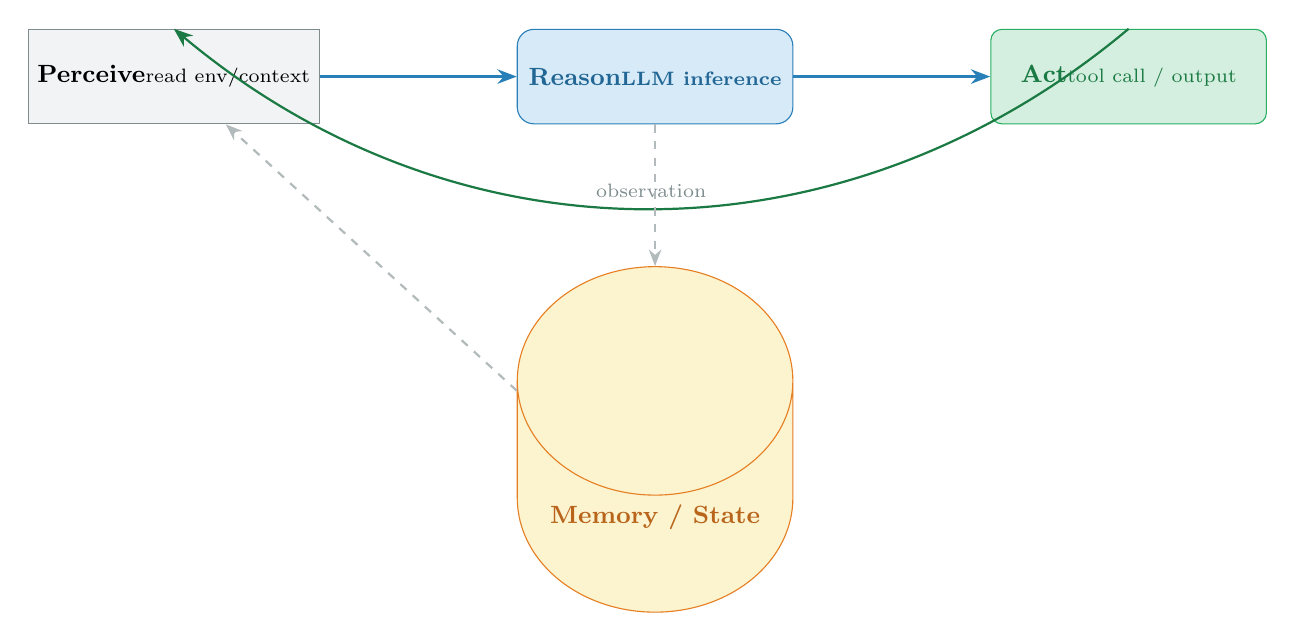
\begin{tikzpicture}[node distance=2cm]
  \node[process, minimum width=3.5cm, minimum height=1.2cm] (percept)
    {\textbf{Perceive}\\{\scriptsize read env/context}};
  \node[agent, minimum width=3.5cm, minimum height=1.2cm, right=2.5cm of percept] (reason)
    {\textbf{Reason}\\{\scriptsize LLM inference}};
  \node[tool, minimum width=3.5cm, minimum height=1.2cm, right=2.5cm of reason] (act)
    {\textbf{Act}\\{\scriptsize tool call / output}};
  \node[store, minimum width=3.5cm, below=1.8cm of reason] (mem)
    {\textbf{Memory / State}};

  \draw[arrowblue] (percept) -- (reason);
  \draw[arrowblue] (reason) -- (act);
  \draw[arrowgreen, bend left=40] (act.north) to
    node[above, font=\scriptsize, color=agentgray]{observation} (percept.north);
  \draw[dasharrow] (reason) -- (mem);
  \draw[dasharrow] (mem) -- (percept);
\end{tikzpicture}
\caption{The core Perceive--Reason--Act loop. Memory feeds context into perception;
actions produce observations that re-enter the loop.}
\label{fig:pra}
\end{figure}

Unlike a simple function call, the loop \emph{repeats}: the outcome of each action
(tool result, error, partial output) is fed back as a new observation, enabling
the agent to react, correct course, or pursue multi-step strategies.

\subsection{Agent Architectures}

Several architectural patterns have emerged:

\subsubsection{ReAct (Reason + Act)}

ReAct~\cite{yao2023react} interleaves chain-of-thought reasoning with action
steps in a single context window:

\begin{lstlisting}[language={},caption=ReAct trace fragment]
Thought: I need to find which section uses the iterative tab.
Action: read_file("sections.json")
Observation: [..., {"id": "15_linear_search", "tab": "iterative"}, ...]
Thought: Section 15 targets iterative tab. I should switch the tab first.
Action: click_tab("iterative")
Observation: {"btnActive": true, "panelVisible": true}
\end{lstlisting}

The model decides \emph{what} to think and \emph{what} to do in the same
generation step. This is simple but vulnerable to long-horizon forgetting and
accumulating errors in the context.

\subsubsection{Plan-and-Execute}

A \emph{planner} agent decomposes the goal into a sequence of steps; separate
\emph{executor} agents carry out each step. The planner may revise the plan
based on executor feedback.

\begin{figure}[h]
\centering
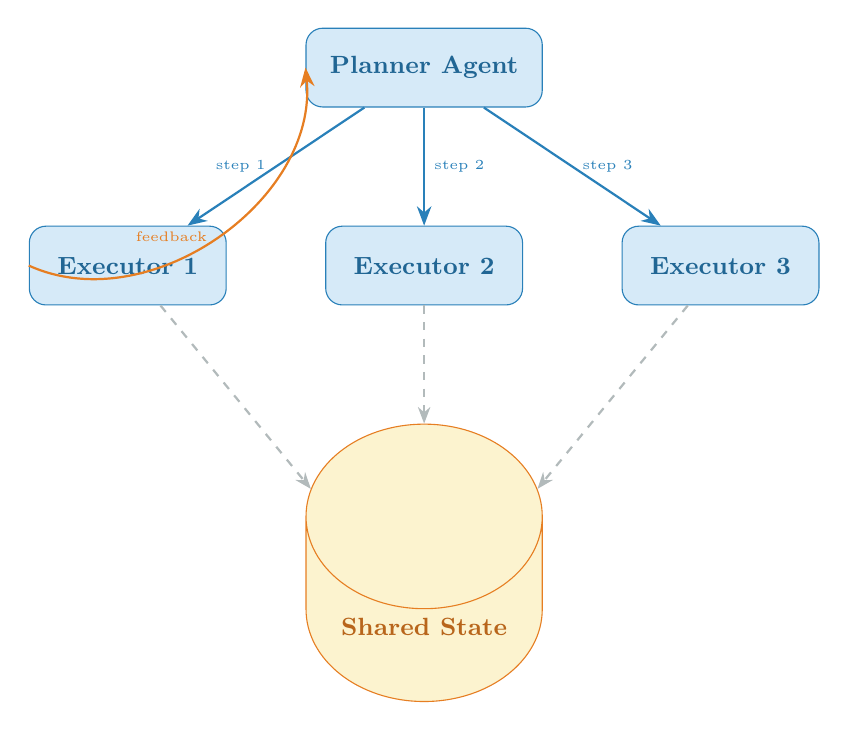
\begin{tikzpicture}[node distance=1.5cm and 3cm]
  \node[agent, minimum width=3cm] (planner) {Planner Agent};
  \node[agent, minimum width=2.5cm, below left=1.5cm and 1cm of planner]  (e1) {Executor 1};
  \node[agent, minimum width=2.5cm, below=1.5cm of planner]               (e2) {Executor 2};
  \node[agent, minimum width=2.5cm, below right=1.5cm and 1cm of planner] (e3) {Executor 3};
  \node[store, minimum width=3cm, below=1.5cm of e2] (state) {Shared State};

  \draw[arrowblue] (planner) -- (e1) node[midway, left, font=\tiny]{step 1};
  \draw[arrowblue] (planner) -- (e2) node[midway, right, font=\tiny]{step 2};
  \draw[arrowblue] (planner) -- (e3) node[midway, right, font=\tiny]{step 3};
  \draw[dasharrow] (e1) -- (state);
  \draw[dasharrow] (e2) -- (state);
  \draw[dasharrow] (e3) -- (state);
  \draw[arroworange, bend right=60] (e1.west) to
    node[left, font=\tiny, color=agentorange]{feedback} (planner.west);
\end{tikzpicture}
\caption{Plan-and-Execute: a planner decomposes goals; executors report back.}
\label{fig:planexec}
\end{figure}

\subsubsection{Reflexion / Self-Critique}

The agent generates an output, then a second (or the same) LLM call evaluates
it and produces a \emph{reflection}. The reflection is stored in memory and
used to improve the next attempt. This directly models the quality-assurance
loop seen in our system.

\subsubsection{Tool-Augmented Agents}

Modern LLMs can invoke structured tools through function-calling APIs. The
model emits a JSON payload; a host process executes the corresponding function
and returns the result. This pattern is the foundation of our pipeline agents.

\begin{figure}[h]
\centering
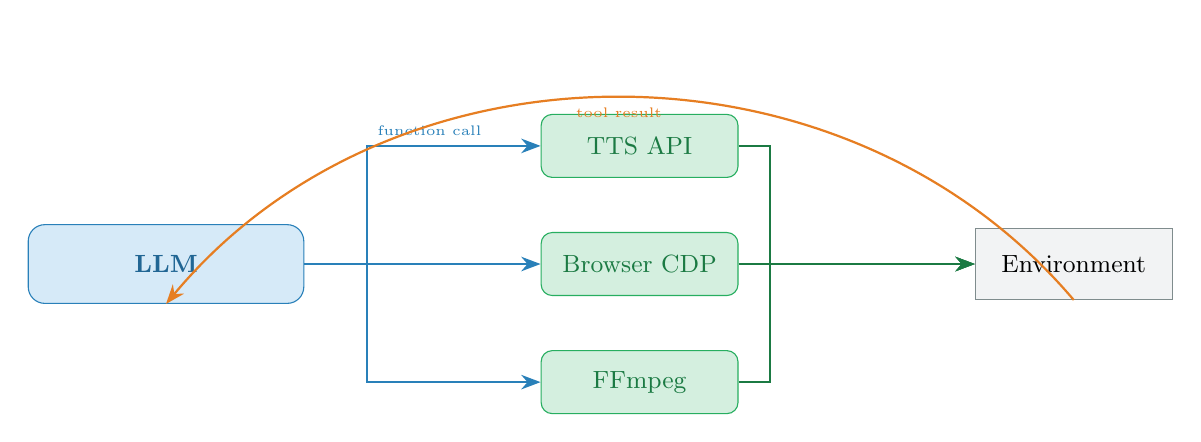
\begin{tikzpicture}
  \node[agent, minimum width=3.5cm] (llm) {LLM};
  \node[tool, minimum width=2.5cm, right=3cm of llm, yshift= 1.5cm] (t1)
    {TTS API};
  \node[tool, minimum width=2.5cm, right=3cm of llm, yshift= 0.0cm] (t2)
    {Browser CDP};
  \node[tool, minimum width=2.5cm, right=3cm of llm, yshift=-1.5cm] (t3)
    {FFmpeg};
  \node[process, minimum width=2.5cm, right=3cm of t2] (env) {Environment};

  \draw[arrowblue] (llm.east) -- ++(0.8,0) |- (t1.west)
    node[midway, above right, font=\tiny]{function call};
  \draw[arrowblue] (llm.east) -- ++(0.8,0) |- (t2.west);
  \draw[arrowblue] (llm.east) -- ++(0.8,0) |- (t3.west);
  \draw[arrowgreen] (t1.east) -- ++(0.4,0) |- (env);
  \draw[arrowgreen] (t2.east) -- (env);
  \draw[arrowgreen] (t3.east) -- ++(0.4,0) |- (env);
  \draw[arroworange, bend right=50] (env.south) to
    node[below, font=\tiny, color=agentorange]{tool result} (llm.south);
\end{tikzpicture}
\caption{Tool-augmented LLM: the model selects tools; a host process executes them.}
\end{figure}

\subsection{Memory Systems}
\label{sec:memory}

Agents typically require multiple layers of memory:

\begin{table}[h]
\centering
\small
\begin{tabular}{@{}llll@{}}
\toprule
\textbf{Type} & \textbf{Scope} & \textbf{Storage} & \textbf{Example} \\
\midrule
In-context    & Current episode & LLM context window & Conversation history \\
External/Episodic & Cross-session & Files, DB & Memory markdown files \\
Procedural    & Permanent & System prompt / code & Agent behaviour rules \\
Semantic      & Domain facts & Vector DB / docs & Course content \\
Working       & Computation & Variable state & Run directory, counters \\
\bottomrule
\end{tabular}
\caption{Memory layers in agentic systems.}
\end{table}

In our pipeline, \emph{external episodic memory} is implemented as Markdown files
in \texttt{.claude/projects/.../memory/}, while \emph{working memory} is the
\texttt{state.json} file persisted in each run directory.

\subsection{Agent Evaluation and Quality Assurance}
\label{sec:agentqa}

A fundamental challenge in agentic systems is verifying that actions produced
the intended outcome. Three strategies exist:

\begin{enumerate}[leftmargin=2em]
  \item \textbf{Deterministic verification} — check ground-truth state directly
        (e.g.\ DOM inspection, file existence, API status code). Fast and exact
        but requires programmatic access to state.
  \item \textbf{LLM-as-judge} — pass the output to a second LLM call that
        evaluates it against a rubric. Flexible but probabilistic; the judge
        can err or be inconsistent across calls on identical input.
  \item \textbf{Human-in-the-loop} — a person reviews and approves the output
        before the pipeline continues. Slowest but highest fidelity.
\end{enumerate}

Our system uses all three. DOM inspection is ground truth for tab correctness
(deterministic); a vision-capable LLM judges screenshot quality (LLM-as-judge);
an optional \texttt{--no-human-review} flag can bypass human checkpoints.

\subsection{Failure Modes in Agentic Systems}

\begin{figure}[h]
\centering
\begin{tikzpicture}[node distance=1.2cm]
  \node[process, fill=agentred!15, draw=agentred, minimum width=4cm] (hf)
    {\textbf{Hallucination / False Positive}\\
     {\scriptsize Agent believes task is done when it is not}};
  \node[process, fill=agentorange!15, draw=agentorange, minimum width=4cm,
        below=0.8cm of hf] (loop)
    {\textbf{Infinite Loop}\\
     {\scriptsize Retry condition never satisfied}};
  \node[process, fill=agentpurple!15, draw=agentpurple, minimum width=4cm,
        below=0.8cm of loop] (cascade)
    {\textbf{Error Cascade}\\
     {\scriptsize Early failure silently propagates downstream}};
  \node[process, fill=agentblue!15, draw=agentblue, minimum width=4cm,
        below=0.8cm of cascade] (overfit)
    {\textbf{Prompt Overfitting}\\
     {\scriptsize Prompt fix works for one case, breaks others}};

  \node[tool, right=3cm of hf, minimum width=3.5cm]   (s1) {DOM ground truth};
  \node[tool, right=3cm of loop, minimum width=3.5cm]  (s2) {Max retry limit};
  \node[tool, right=3cm of cascade, minimum width=3.5cm](s3) {State checkpoints};
  \node[tool, right=3cm of overfit, minimum width=3.5cm](s4) {Engineering fix};

  \draw[arrowgreen] (s1) -- (hf);
  \draw[arrowgreen] (s2) -- (loop);
  \draw[arrowgreen] (s3) -- (cascade);
  \draw[arrowgreen] (s4) -- (overfit);

  \node[font=\small\bfseries, color=agentred,  left=0.2cm of hf]     {\faExclamationTriangle};
  \node[font=\small\bfseries, color=agentorange, left=0.2cm of loop]  {\faExclamationTriangle};
  \node[font=\small\bfseries, color=agentpurple, left=0.2cm of cascade]{\faExclamationTriangle};
  \node[font=\small\bfseries, color=agentblue, left=0.2cm of overfit] {\faExclamationTriangle};
\end{tikzpicture}
\caption{Common agentic failure modes (left) and mitigations used in this system (right).}
\end{figure}

% =============================================================================
\section{Multi-Agent Orchestration}
\label{sec:multiagent}
% =============================================================================

\subsection{Orchestrator–Worker Pattern}

The most common multi-agent topology is hierarchical: an \emph{orchestrator}
maintains the high-level goal and delegates subtasks to specialised \emph{workers}.

\begin{figure}[h]
\centering
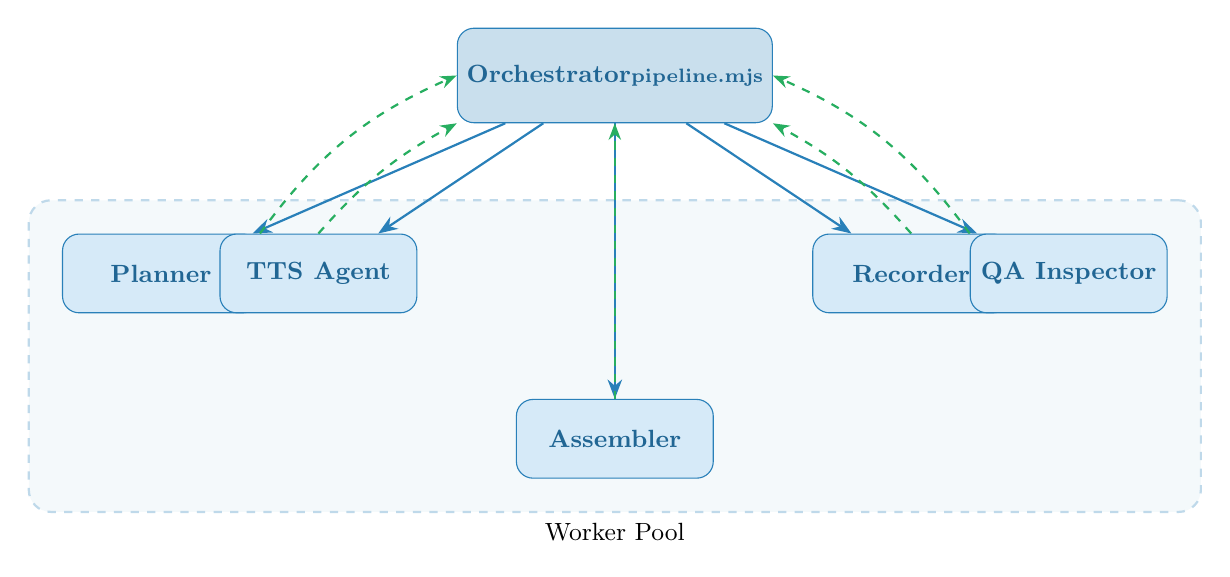
\begin{tikzpicture}[node distance=1.4cm and 1.8cm]
  \node[agent, fill=agentblue!25, draw=agentblue, minimum width=4cm,
        minimum height=1.2cm] (orch) {\textbf{Orchestrator}\\{\scriptsize pipeline.mjs}};

  \node[agent, below left=1.4cm and 2.5cm of orch, minimum width=2.5cm]  (w1)
    {Planner};
  \node[agent, below left=1.4cm and 0.5cm of orch, minimum width=2.5cm]  (w2)
    {TTS Agent};
  \node[agent, below right=1.4cm and 0.5cm of orch, minimum width=2.5cm] (w3)
    {Recorder};
  \node[agent, below right=1.4cm and 2.5cm of orch, minimum width=2.5cm] (w4)
    {QA Inspector};
  \node[agent, below=3.5cm of orch, minimum width=2.5cm]                 (w5)
    {Assembler};

  \draw[arrowblue] (orch) -- (w1);
  \draw[arrowblue] (orch) -- (w2);
  \draw[arrowblue] (orch) -- (w3);
  \draw[arrowblue] (orch) -- (w4);
  \draw[arrowblue] (orch) -- (w5);

  \draw[dasharrow, color=agentgreen] (w1.north east) to[bend left=15] (orch.west);
  \draw[dasharrow, color=agentgreen] (w2.north)      to[bend left=10] (orch.south west);
  \draw[dasharrow, color=agentgreen] (w3.north)      to[bend right=10](orch.south east);
  \draw[dasharrow, color=agentgreen] (w4.north west) to[bend right=15](orch.east);
  \draw[dasharrow, color=agentgreen] (w5.north)      -- (orch.south);

  \begin{scope}[on background layer]
    \node[groupbox, draw=agentblue!30, fill=agentblue!5,
          fit=(w1)(w2)(w3)(w4)(w5), label=below:{\small Worker Pool}] {};
  \end{scope}
\end{tikzpicture}
\caption{Orchestrator–worker topology used in the lecture production pipeline.}
\label{fig:orchworker}
\end{figure}

\subsection{Inter-Agent Communication Channels}

Agents in our system communicate through three channels:

\begin{enumerate}[leftmargin=2em]
  \item \textbf{Direct function call} --- synchronous; the orchestrator calls a
        worker function and awaits its return value. Used for TTS, recording, QA.
  \item \textbf{Shared file state} --- \texttt{state.json} and the run directory
        act as a blackboard. Any agent can read or write; the orchestrator coordinates
        access. Enables crash recovery.
  \item \textbf{LLM context injection} --- worker prompts are constructed by the
        orchestrator, embedding relevant state (section config, previous QA scores,
        tab state) before calling the LLM API.
\end{enumerate}

\subsection{Parallelism and Sequential Constraints}

\begin{figure}[h]
\centering
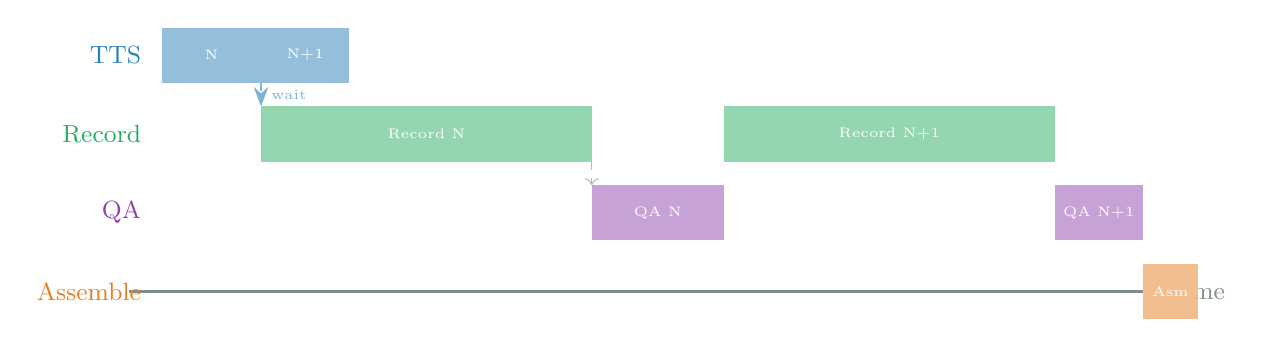
\begin{tikzpicture}[x=1.4cm, y=1cm]
  % Timeline
  \draw[thick, ->, color=agentgray] (-0.2,0) -- (9.2,0)
    node[right, font=\small]{time};

  % Row labels
  \node[font=\small, left, color=agentblue]   at (0, 3) {TTS};
  \node[font=\small, left, color=agentgreen]  at (0, 2) {Record};
  \node[font=\small, left, color=agentpurple] at (0, 1) {QA};
  \node[font=\small, left, color=agentorange] at (0, 0) {Assemble};

  % Section N
  \fill[agentblue!50]   (0.1, 2.65) rectangle (1.0, 3.35);
  \fill[agentgreen!50]  (1.0, 1.65) rectangle (4.0, 2.35);
  \fill[agentpurple!50] (4.0, 0.65) rectangle (5.2, 1.35);

  % Section N+1 (TTS can overlap with recording of N)
  \fill[agentblue!50]   (1.0, 2.65) rectangle (1.8, 3.35)
    node[midway, font=\tiny, color=white]{N+1};
  \fill[agentgreen!50]  (5.2, 1.65) rectangle (8.2, 2.35);
  \fill[agentpurple!50] (8.2, 0.65) rectangle (9.0, 1.35);

  % Assembly (after all sections)
  \fill[agentorange!50] (9.0, -0.35) rectangle (9.5, 0.35);

  % Labels
  \node[font=\tiny, color=white] at (0.55, 3) {N};
  \node[font=\tiny, color=white] at (2.5,  2) {Record N};
  \node[font=\tiny, color=white] at (4.6,  1) {QA N};
  \node[font=\tiny, color=white] at (6.7,  2) {Record N+1};
  \node[font=\tiny, color=white] at (8.6,  1) {QA N+1};
  \node[font=\tiny, color=white] at (9.25, 0) {Asm};

  % Dependency arrows
  \draw[arrowblue, dashed, color=agentblue!60]
    (1.0, 2.65) -- (1.0, 2.35) node[midway, right, font=\tiny]{wait};

  \draw[->, dashed, color=agentgray!60]
    (4.0, 1.65) -- (4.0, 1.35);
\end{tikzpicture}
\caption{Temporal dependencies in the pipeline. TTS for section $N+1$ can overlap
with recording of $N$; assembly is strictly after all sections.}
\label{fig:timeline}
\end{figure}

% =============================================================================
\section{Part II: The Lecture Production Pipeline}
\label{sec:ouroverview}
% =============================================================================

\subsection{System Overview and Motivation}

The system automates the production of narrated, screen-recorded lecture videos
from an interactive HTML educational tool. The goal is to replace the hours of
manual effort required to record, narrate, and edit a lecture with a fully
agentic pipeline that: (a) generates narration scripts, (b) synthesises speech,
(c) controls the browser tool to show the right content at the right time,
(d) captures synchronized video, (e) performs quality assurance at each step,
and (f) assembles the final video.

\begin{figure}[h]
\centering
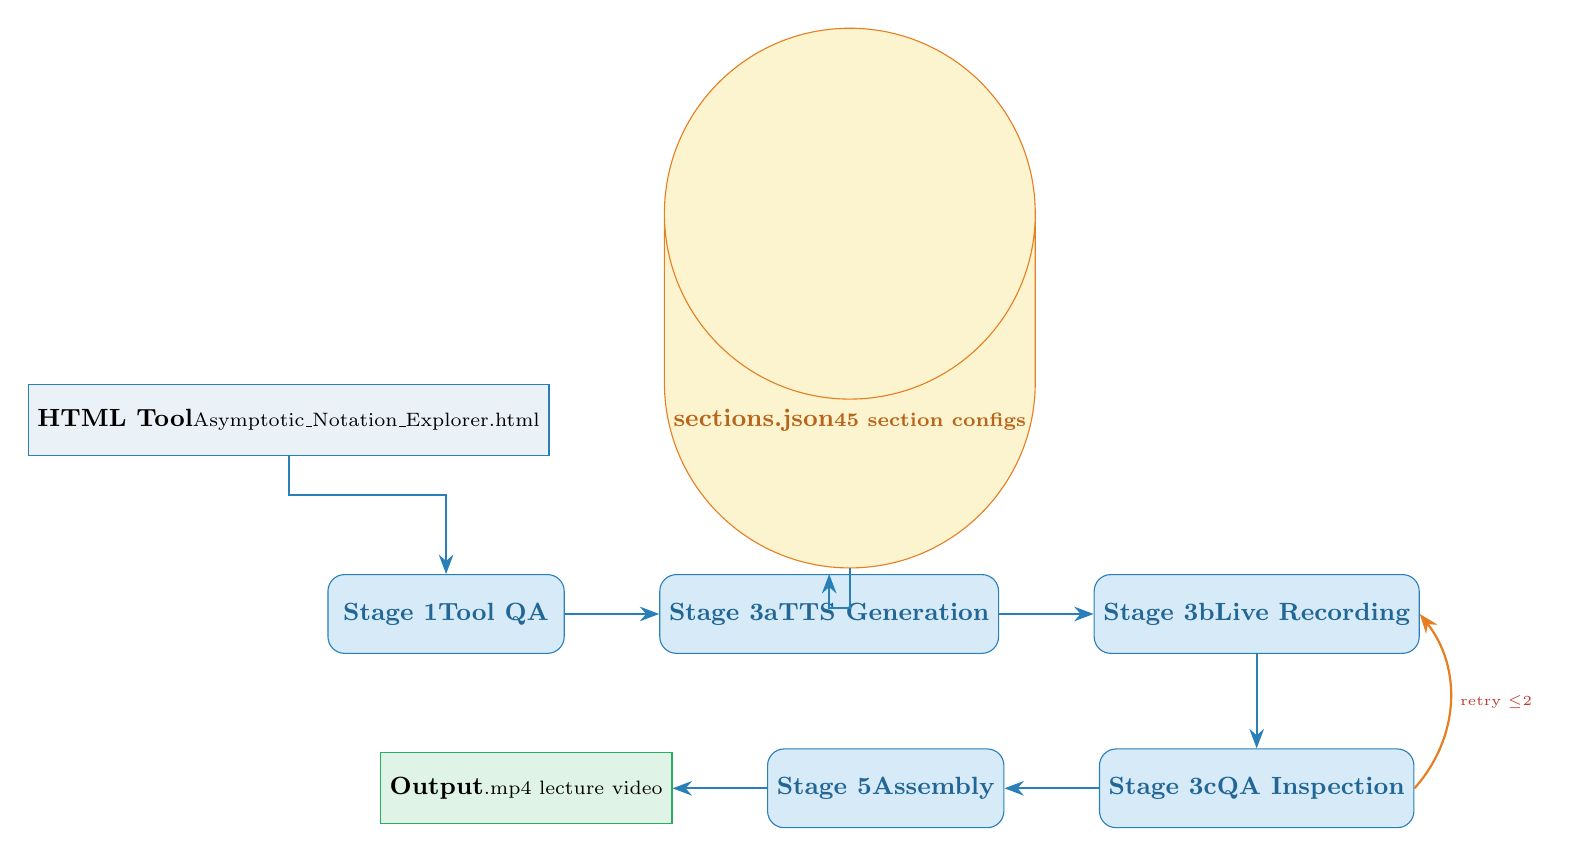
\begin{tikzpicture}[node distance=0.8cm and 0.4cm]
  % Input
  \node[process, minimum width=3.5cm, fill=agentblue!10, draw=agentblue] (html)
    {\textbf{HTML Tool}\\{\scriptsize Asymptotic\_Notation\_Explorer.html}};
  \node[store, right=1.5cm of html, minimum width=2.8cm] (cfg)
    {\textbf{sections.json}\\{\scriptsize 45 section configs}};

  % Stage boxes
  \node[agent, below=1.5cm of html, xshift=2cm, minimum width=3cm] (plan)
    {Stage 1\\Tool QA};
  \node[agent, right=1.2cm of plan, minimum width=3cm] (tts)
    {Stage 3a\\TTS Generation};
  \node[agent, right=1.2cm of tts, minimum width=3cm] (rec)
    {Stage 3b\\Live Recording};
  \node[agent, below=1.2cm of rec, minimum width=3cm] (qa)
    {Stage 3c\\QA Inspection};
  \node[agent, left=1.2cm of qa, minimum width=3cm] (asm)
    {Stage 5\\Assembly};
  \node[process, left=1.2cm of asm, minimum width=3cm, fill=agentgreen!15,
        draw=agentgreen] (out)
    {\textbf{Output}\\{\scriptsize .mp4 lecture video}};

  % Arrows
  \draw[arrowblue] (html.south) -- ++(0,-0.5) -| (plan.north);
  \draw[arrowblue] (cfg.south)  -- ++(0,-0.5) -| (tts.north);
  \draw[arrowblue] (plan) -- (tts);
  \draw[arrowblue] (tts) -- (rec);
  \draw[arrowblue] (rec.south) -- (qa.north);
  \draw[arrowblue] (qa) -- (asm);
  \draw[arrowblue] (asm) -- (out);

  % Retry loop
  \draw[arroworange, bend right=40] (qa.east)
    to node[right, font=\tiny, color=agentred]{retry $\leq$2} (rec.east);
\end{tikzpicture}
\caption{High-level pipeline stages.}
\label{fig:pipeline}
\end{figure}

\subsection{Input: Interactive HTML Tool}

The tool is a single-page application
(\texttt{Asymptotic\_Notation\_Explorer.html}) implementing five tabs:

\begin{table}[h]
\centering\small
\begin{tabular}{@{}lll@{}}
\toprule
\textbf{Tab} & \textbf{\texttt{data-mod}} & \textbf{Content} \\
\midrule
Notation Guide     & \texttt{notations}  & Big-O/Ω/Θ definitions, comparison charts \\
Iterative Analysis & \texttt{iterative}  & Step counters, complexity charts per sort \\
Recursive Analysis & \texttt{recursive}  & Recursion trees, merge/quick/binary search \\
Proof Builder      & \texttt{prover}     & Interactive formal proof construction \\
Challenge Mode     & \texttt{challenge}  & Practice problems with feedback \\
\bottomrule
\end{tabular}
\caption{The five tabs of the interactive HTML tool.}
\end{table}

A critical engineering issue was discovered: space-utilisation fixes had added
\texttt{display:flex} as an \emph{inline style} to all tab panels. Because
inline styles have higher CSS specificity than class rules, the class
\texttt{.module\{display:none\}} was overridden, making all panels simultaneously
visible. The fix was to explicitly set \texttt{display:none} in the inline style
of inactive panels.

\subsection{Stage 1: Tool Quality Assurance}

Before any recording, a vision-capable LLM inspects a screenshot of the loaded
tool and evaluates it against a structured rubric (viewport overflow, interactive
elements, tab accessibility). If the score falls below 75/100, the tool-fixer
agent is invoked to patch the HTML.

\subsection{Stage 3: Per-Section Recording Loop}
\label{sec:recording}

This is the core of the pipeline. For each of the 45 sections:

\begin{figure}[h]
\centering
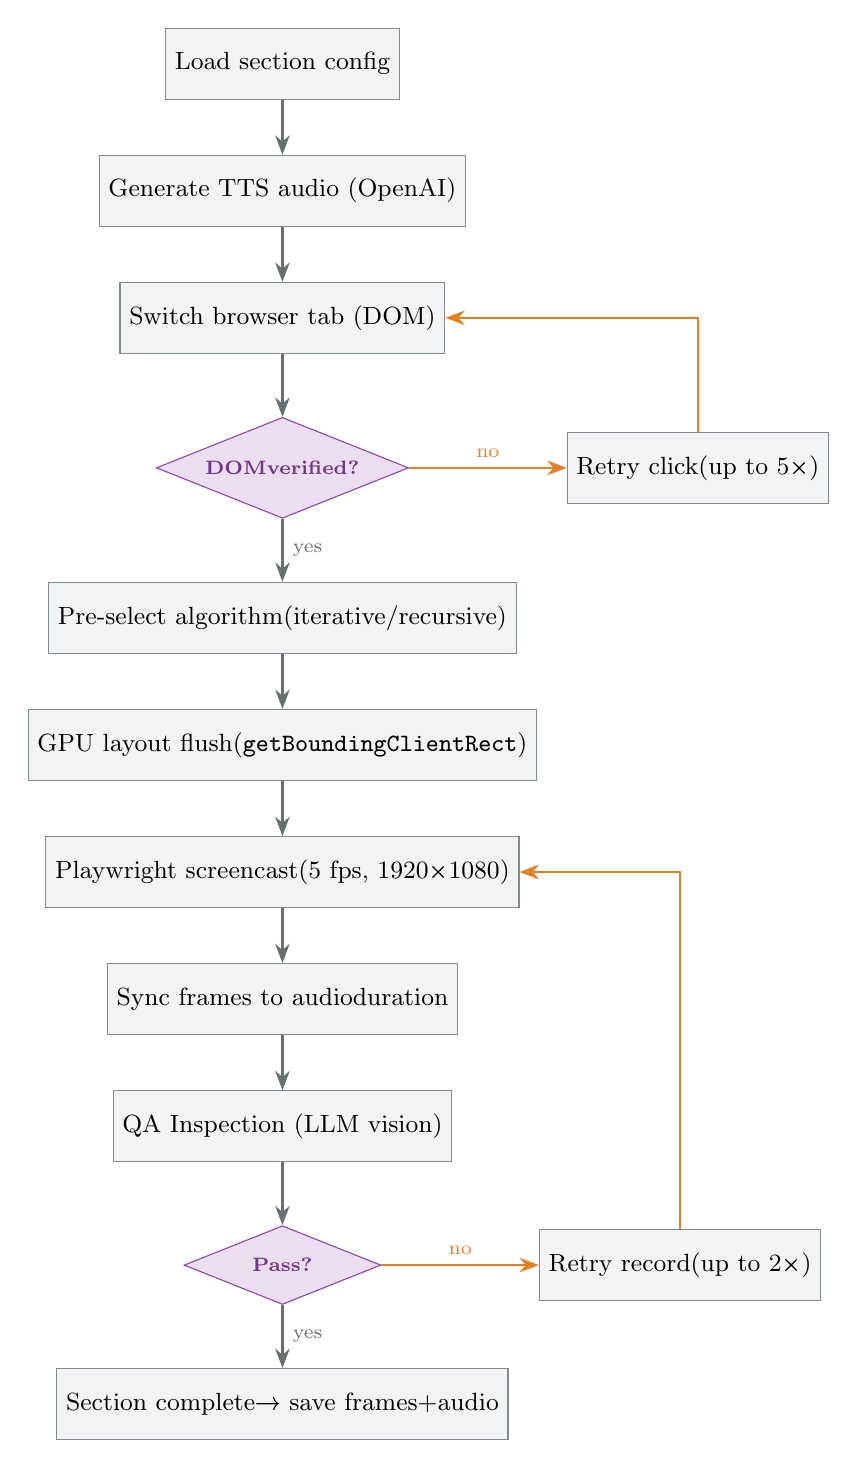
\begin{tikzpicture}[node distance=1cm and 0.5cm,
                    every node/.style={font=\small}]
  \node[process] (start) {Load section config};
  \node[process, below=0.7cm of start] (tts) {Generate TTS audio (OpenAI)};
  \node[process, below=0.7cm of tts] (tab) {Switch browser tab (DOM)};
  \node[decision, below=0.8cm of tab, aspect=2.5] (domcheck)
    {DOM\\verified?};
  \node[process, right=2cm of domcheck] (retry_tab)
    {Retry click\\(up to 5×)};
  \node[process, below=0.8cm of domcheck] (algo)
    {Pre-select algorithm\\(iterative/recursive)};
  \node[process, below=0.7cm of algo] (flush)
    {GPU layout flush\\(\texttt{getBoundingClientRect})};
  \node[process, below=0.7cm of flush] (screencast)
    {Playwright screencast\\(5 fps, 1920×1080)};
  \node[process, below=0.7cm of screencast] (sync)
    {Sync frames to audio\\duration};
  \node[process, below=0.7cm of sync] (qa) {QA Inspection (LLM vision)};
  \node[decision, below=0.8cm of qa, aspect=2.5] (pass)
    {Pass?};
  \node[process, right=2cm of pass] (retry)
    {Retry record\\(up to 2×)};
  \node[process, below=0.8cm of pass] (done)
    {Section complete\\→ save frames+audio};

  \draw[arrow] (start) -- (tts);
  \draw[arrow] (tts) -- (tab);
  \draw[arrow] (tab) -- (domcheck);
  \draw[arrow] (domcheck) -- node[right]{\scriptsize yes} (algo);
  \draw[arroworange] (domcheck) -- node[above]{\scriptsize no} (retry_tab);
  \draw[arroworange] (retry_tab) |- (tab);
  \draw[arrow] (algo) -- (flush);
  \draw[arrow] (flush) -- (screencast);
  \draw[arrow] (screencast) -- (sync);
  \draw[arrow] (sync) -- (qa);
  \draw[arrow] (qa) -- (pass);
  \draw[arrow] (pass) -- node[right]{\scriptsize yes} (done);
  \draw[arroworange] (pass) -- node[above]{\scriptsize no} (retry);
  \draw[arroworange] (retry) |- (screencast);
\end{tikzpicture}
\caption{Detailed flow for each section in Stage 3.}
\label{fig:sectionflow}
\end{figure}

\subsubsection{Tab Switching: Engineering vs Prompt-Based Verification}

The tab-switching problem illustrates a fundamental principle: \emph{prompt-based
verification cannot replace engineering verification}.

Earlier versions asked the QA LLM to confirm the correct tab was showing. The LLM
produced false positives (the Notation Guide header also appears as a panel title,
confusing the vision model). The engineering solution is a DOM query executed in
the page JavaScript context:

\begin{lstlisting}[language=JavaScript, caption=DOM-verified tab check]
const state = await page.evaluate((tab) => {
  const btn   = document.querySelector(`.tab[data-mod="${tab}"]`);
  const panel = document.querySelector(`#viz-${tab}`);
  return {
    btnActive:    btn?.classList.contains('active') ?? false,
    panelVisible: window.getComputedStyle(panel).display !== 'none'
  };
}, expectedTab);
// Both must be true before recording starts
if (!state.btnActive || !state.panelVisible) { /* retry click */ }
\end{lstlisting}

This is deterministic: it queries the live render tree, not a screenshot
interpretation.

\subsubsection{GPU-Accelerated Rendering}

The original implementation used Playwright's default \texttt{chrome-headless-shell}
binary. This binary forces \texttt{--disable-gpu} internally: CSS display changes
applied in the DOM were not flushed to the compositor before screenshots were
taken, causing stale frames to be captured despite correct DOM state.

The fix uses \texttt{channel: 'chrome'} with \texttt{headless: true}, which
invokes the real Chrome binary in "new headless" mode (introduced Chrome~112).
This engages the full GPU compositing pipeline (Metal on Apple Silicon):

\begin{figure}[h]
\centering
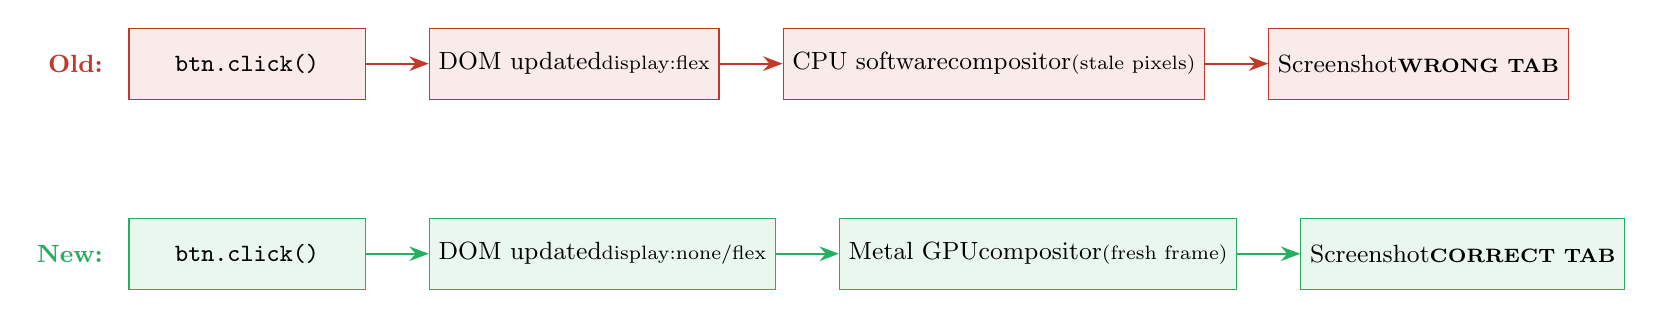
\begin{tikzpicture}
  % Old path
  \node[process, draw=agentred, fill=agentred!10, minimum width=3cm] (old_tab)
    {\texttt{btn.click()}};
  \node[process, draw=agentred, fill=agentred!10, minimum width=3cm,
        right=0.8cm of old_tab] (old_dom)
    {DOM updated\\{\scriptsize display:flex}};
  \node[process, draw=agentred, fill=agentred!10, minimum width=3.5cm,
        right=0.8cm of old_dom] (old_comp)
    {CPU software\\compositor\\{\scriptsize (stale pixels)}};
  \node[process, draw=agentred, fill=agentred!10, minimum width=2.5cm,
        right=0.8cm of old_comp] (old_shot)
    {Screenshot\\{\scriptsize \textbf{WRONG TAB}}};

  \draw[arrow, color=agentred] (old_tab) -- (old_dom);
  \draw[arrow, color=agentred] (old_dom) -- (old_comp);
  \draw[arrow, color=agentred] (old_comp) -- (old_shot);
  \node[font=\small\bfseries, color=agentred, left=0.2cm of old_tab]
    {Old:};

  % New path
  \node[process, draw=agentgreen, fill=agentgreen!10, minimum width=3cm,
        below=1.5cm of old_tab] (new_tab)
    {\texttt{btn.click()}};
  \node[process, draw=agentgreen, fill=agentgreen!10, minimum width=3cm,
        right=0.8cm of new_tab] (new_dom)
    {DOM updated\\{\scriptsize display:none/flex}};
  \node[process, draw=agentgreen, fill=agentgreen!10, minimum width=3.5cm,
        right=0.8cm of new_dom] (new_comp)
    {Metal GPU\\compositor\\{\scriptsize (fresh frame)}};
  \node[process, draw=agentgreen, fill=agentgreen!10, minimum width=2.5cm,
        right=0.8cm of new_comp] (new_shot)
    {Screenshot\\{\scriptsize \textbf{CORRECT TAB}}};

  \draw[arrow, color=agentgreen] (new_tab) -- (new_dom);
  \draw[arrow, color=agentgreen] (new_dom) -- (new_comp);
  \draw[arrow, color=agentgreen] (new_comp) -- (new_shot);
  \node[font=\small\bfseries, color=agentgreen, left=0.2cm of new_tab]
    {New:};
\end{tikzpicture}
\caption{Old (headless-shell, software rendering) vs new (real Chrome, Metal GPU)
         rendering pipeline. The GPU path flushes composited frames before
         screenshot capture.}
\label{fig:gpu}
\end{figure}

\subsubsection{HTTP Server vs \texttt{file://} URL}

Serving the tool over a local HTTP server (Node.js built-in \texttt{http} module,
random port) resolves several \texttt{file://} URL limitations:

\begin{itemize}[leftmargin=2em]
  \item \texttt{waitUntil: 'networkidle'} is meaningful (real HTTP requests exist)
  \item \texttt{Cache-Control: no-store} ensures each page load is fresh
  \item Query-string parameters and reload semantics behave as expected
\end{itemize}

\begin{lstlisting}[language=JavaScript, caption=Embedded HTTP server]
function startToolServer(toolPath) {
  const server = createServer(async (req, res) => {
    const filePath = resolveFilePath(req.url, toolPath);
    res.writeHead(200, {
      'Content-Type': mimeType(filePath),
      'Cache-Control': 'no-store'       // always fresh
    });
    createReadStream(filePath).pipe(res);
  });
  server.listen(0, '127.0.0.1', () => {  // port 0 = OS assigns free port
    resolveP({ server, url: `http://127.0.0.1:${server.address().port}/` });
  });
}
\end{lstlisting}

\subsection{Stage 3c: Quality Assurance Agent}
\label{sec:qa}

After each section is recorded, a vision-capable LLM receives a sample frame and
evaluates a structured checklist:

\begin{table}[h]
\centering\small
\begin{tabular}{@{}llll@{}}
\toprule
\textbf{Check} & \textbf{Type} & \textbf{Hard fail?} & \textbf{Score cap} \\
\midrule
\texttt{correct\_tab}      & DOM (ground truth override) & Yes & 0 if false \\
\texttt{text\_readable}    & LLM vision                  & No  & Warning only \\
\texttt{pointer\_visible}  & LLM vision                  & No  & $-$10 pts \\
\texttt{content\_matches}  & LLM vision                  & Yes & 0 if false \\
\texttt{right\_panel\_active} & LLM vision               & No  & $\leq 50$ if false \\
\texttt{space\_utilized}   & LLM vision                  & No  & $-$15 pts \\
\bottomrule
\end{tabular}
\caption{QA checklist items, verification method, and scoring impact.}
\end{table}

A key design decision is that \texttt{correct\_tab} is \emph{overridden} with the
DOM-verified result from \texttt{page.evaluate()}, regardless of what the LLM
judge reports. This prevents vision hallucinations from masking a real tab error.

\subsubsection{Pitfall: Retry Loops on Unresolvable Failures}

An early version made \texttt{text\_readable} a hard-fail trigger. Chart axis tick
labels are rendered at ~10px by Chart.js regardless of retries. This caused every
chart section to exhaust all retries (recording the same content 3 times), wasting
$3 \times 30\text{s} \times 30\text{ sections} \approx 45$ minutes per run. The fix:
only retry on failures that are \emph{causal} (wrong tab, content mismatch); style
issues become warnings.

\subsection{Stage 5: Video Assembly}

After all sections complete, \texttt{assembleFullLecture()} uses FFmpeg to:

\begin{enumerate}[leftmargin=2em]
  \item Convert each section's frame sequence + audio into a per-section
        \texttt{.mp4} segment (H.264, VideoToolbox hardware encoder on Apple Silicon)
  \item Concatenate all segments using FFmpeg's \texttt{concat} demuxer
  \item Optionally burn subtitle bars via \texttt{drawtext} filter
\end{enumerate}

\begin{figure}[h]
\centering
\begin{tikzpicture}
  \foreach \i/\name in {0/S1, 1.5/S2, 3/..., 4.5/S45} {
    \node[process, minimum width=1.2cm, minimum height=1.8cm,
          draw=agentblue, fill=agentblue!10]
      at (\i*1.4, 1) {\small\name\\{\tiny frames}\\{\tiny +audio}};
  }
  \node[font=\Large, color=agentgray] at (3.5*1.4, 1) {$\cdots$};

  \node[tool, minimum width=2cm, below=1.2cm of {(3*1.4,1)}] (ffmpeg)
    {FFmpeg\\VideoToolbox};

  \node[process, fill=agentgreen!15, draw=agentgreen, minimum width=4cm,
        below=1.2cm of ffmpeg] (out)
    {\textbf{Lecture.mp4}\\{\scriptsize 1920×1080 H.264}};

  \draw[arrowblue] (0*1.4, 0.1) -- (ffmpeg.north west);
  \draw[arrowblue] (1.5*1.4, 0.1) -- (ffmpeg.north);
  \draw[arrowblue] (4.5*1.4, 0.1) -- (ffmpeg.north east);
  \draw[arrowgreen] (ffmpeg) -- (out);
\end{tikzpicture}
\caption{Assembly stage: per-section frame sequences are encoded and concatenated.}
\end{figure}

% =============================================================================
\section{State Management and Crash Recovery}
\label{sec:state}
% =============================================================================

The pipeline writes a \texttt{state.json} file after each section completes.
This enables resuming interrupted runs:

\begin{lstlisting}[language=JavaScript, caption=State persistence pattern]
// After each section
state.data.completedSections.push(sectionId);
state.data.sections[sectionId] = {
  framesDir, audioPath, qaScore, qaChecklist, timestamp
};
await state.save();  // atomic write to state.json
\end{lstlisting}

On restart, the pipeline skips sections already present in
\texttt{state.data.completedSections}, making every run \emph{idempotent} with
respect to completed work.

% =============================================================================
\section{Lessons Learned and Design Principles}
\label{sec:lessons}
% =============================================================================

\subsection{Principle 1: Engineering Verification Over Prompt Verification}

Whenever the correctness of an action can be verified programmatically (DOM
state, file existence, HTTP status), do so. LLM-as-judge is powerful but
non-deterministic: the same frame can receive different scores across calls.
Reserve LLM judgement for inherently subjective evaluations (readability,
clarity, pacing).

\subsection{Principle 2: Identify the Root Cause Layer}

The wrong-tab bug existed at three layers simultaneously:
\begin{enumerate}[leftmargin=2em]
  \item HTML: \texttt{display:flex} inline style overriding CSS \texttt{display:none}
  \item Rendering: software compositor not flushing CSS changes before screenshot
  \item Verification: LLM judge misidentifying the active tab from visual context
\end{enumerate}
Fixing only one layer left the others as latent failures. The permanent fix
addressed all three.

\subsection{Principle 3: Bound Retry Behaviour}

Every retry loop must have:
\begin{itemize}[leftmargin=2em]
  \item A maximum iteration count
  \item A check that the failure is \emph{resolvable by retrying} (idempotent
        retries on a deterministically failing condition are pure waste)
  \item A fallback that logs and continues rather than hanging
\end{itemize}

\subsection{Principle 4: Separate Concerns Between Agents}

Each agent has one responsibility:
\begin{itemize}[leftmargin=2em]
  \item TTS Agent: text → audio file
  \item Recorder: browser state + audio → frame sequence
  \item QA Inspector: frame sample → structured quality report
  \item Assembler: frames + audio → \texttt{.mp4} segments → final video
\end{itemize}

The orchestrator (\texttt{pipeline.mjs}) contains the control logic but no
domain implementation. This separation makes each component testable and
replaceable independently.

\subsection{Principle 5: Use Infrastructure, Not Workarounds}

Serving the HTML tool over a real HTTP server (instead of \texttt{file://}
URLs with reload hacks) is an example of using the right infrastructure. Each
workaround applied to a \texttt{file://} URL (\texttt{cache-bust} query strings,
forced \texttt{page.reload()}, extended timeouts) was a symptom of using the
wrong transport. One infrastructure change eliminated all of them.

% =============================================================================
\section{System Architecture Summary}
% =============================================================================

\begin{figure}[h]
\centering
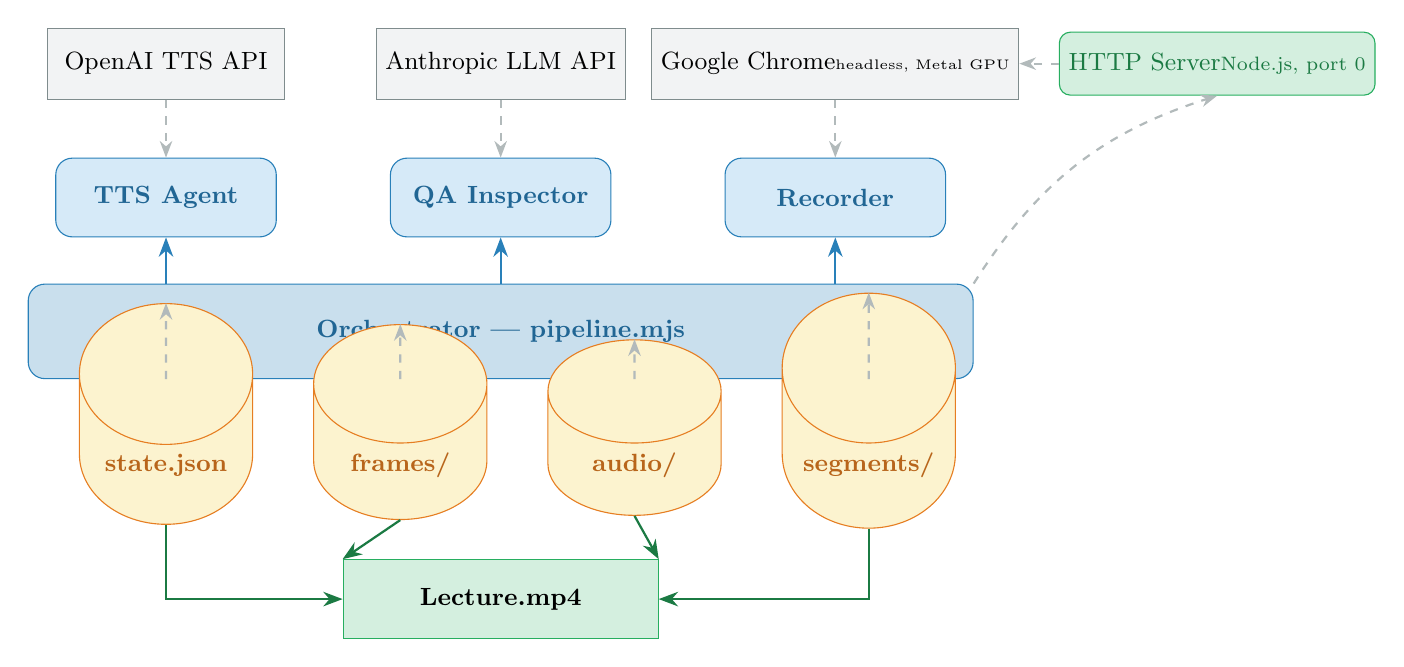
\begin{tikzpicture}[x=0.85cm, y=0.85cm]
  % ── Layer 0: External ────────────────────────────────────────────
  \node[process, minimum width=3cm, draw=agentgray, fill=lightgray] (openai)
    at (0, 8) {\small OpenAI TTS API};
  \node[process, minimum width=3cm, draw=agentgray, fill=lightgray] (anthropic)
    at (5, 8) {\small Anthropic LLM API};
  \node[process, minimum width=3cm, draw=agentgray, fill=lightgray] (chrome)
    at (10, 8) {\small Google Chrome\\{\tiny headless, Metal GPU}};

  % ── Layer 1: Agents ──────────────────────────────────────────────
  \node[agent, minimum width=2.8cm] (tts_agent)
    at (0, 6) {TTS Agent};
  \node[agent, minimum width=2.8cm] (qa_agent)
    at (5, 6) {QA Inspector};
  \node[agent, minimum width=2.8cm] (rec_agent)
    at (10, 6) {Recorder};

  % ── Layer 2: Orchestrator ─────────────────────────────────────────
  \node[agent, fill=agentblue!25, draw=agentblue,
        minimum width=12cm, minimum height=1.2cm] (orch)
    at (5, 4) {\textbf{Orchestrator} — pipeline.mjs};

  % ── Layer 3: Storage ──────────────────────────────────────────────
  \node[store, minimum width=2.2cm] (state)   at (0, 2)  {state.json};
  \node[store, minimum width=2.2cm] (frames)  at (3.5, 2){frames/};
  \node[store, minimum width=2.2cm] (audio)   at (7, 2)  {audio/};
  \node[store, minimum width=2.2cm] (segs)    at (10.5, 2){segments/};

  % ── Layer 4: Output ───────────────────────────────────────────────
  \node[process, minimum width=4cm, draw=agentgreen, fill=lightgreen,
        minimum height=1cm] (output) at (5, 0) {\textbf{Lecture.mp4}};

  % ── Connections ───────────────────────────────────────────────────
  \draw[dasharrow] (openai)   -- (tts_agent);
  \draw[dasharrow] (anthropic)-- (qa_agent);
  \draw[dasharrow] (chrome)   -- (rec_agent);

  \draw[arrowblue] (orch.north -| tts_agent) -- (tts_agent.south);
  \draw[arrowblue] (orch.north -| qa_agent)  -- (qa_agent.south);
  \draw[arrowblue] (orch.north -| rec_agent) -- (rec_agent.south);

  \draw[dasharrow] (orch.south -| state)  -- (state.north);
  \draw[dasharrow] (orch.south -| frames) -- (frames.north);
  \draw[dasharrow] (orch.south -| audio)  -- (audio.north);
  \draw[dasharrow] (orch.south -| segs)   -- (segs.north);

  \draw[arrowgreen] (state.south)  |- (output.west);
  \draw[arrowgreen] (frames.south) -- (output.north west);
  \draw[arrowgreen] (audio.south)  -- (output.north east);
  \draw[arrowgreen] (segs.south)   |- (output.east);

  % ── HTTP server annotation ───────────────────────────────────────
  \node[tool, minimum width=2.5cm, right=0.5cm of chrome] (http)
    {HTTP Server\\{\scriptsize Node.js, port 0}};
  \draw[dasharrow] (http.west) -- (chrome.east);
  \draw[dasharrow, bend left=20] (orch.north east) to (http.south);
\end{tikzpicture}
\caption{Full system architecture showing agents, external services, storage,
         and data flow.}
\label{fig:arch}
\end{figure}

% =============================================================================
\section{Conclusion}
% =============================================================================

The lecture production pipeline demonstrates that agentic systems can automate
complex, multi-step creative and technical workflows when designed with the
following principles in mind: clear separation of agent responsibilities,
deterministic verification where possible, bounded retry behaviour, proper
infrastructure rather than workarounds, and persistent state for crash recovery.

The recurring tab-switching bug---which caused hours of wasted runs---was
ultimately a lesson in the difference between \emph{symptoms} and
\emph{root causes}. Three separate layers each needed fixing. An agent that
only patches the symptom (prompt-level instructions to ``switch to the correct
tab'') cannot fix a rendering pipeline deficiency. The engineering solution
(HTML inline styles + DOM verification + GPU compositor) is permanent and
unconditional.

Future extensions to this system could include:
\begin{itemize}[leftmargin=2em]
  \item Per-section video assembly immediately after recording for mid-run
        human or agent inspection
  \item Parallel TTS pre-generation for all sections before recording begins
  \item A scheduling agent to run overnight with remote status notifications
  \item Extension to other interactive HTML tools beyond the notation explorer
\end{itemize}

% =============================================================================
\section{Cost Analysis: Claude API vs.\ Claude Code}
\label{sec:cost}
% =============================================================================

\subsection{The API Cost Problem}

Building the lecture production pipeline with direct calls to the Anthropic API
(Claude API) incurs real, per-token costs at every stage. A single full run of
the 45-section pipeline exercises the LLM multiple times per section:

\begin{table}[h]
\centering\small
\begin{tabular}{@{}llrr@{}}
\toprule
\textbf{Agent} & \textbf{Model} & \textbf{Calls/section} & \textbf{Tokens/call (est.)} \\
\midrule
QA Inspector (vision)  & claude-sonnet-4-6 & 1--3 & $\sim$2\,000 input + 400 output \\
Section Planner        & claude-opus-4-6   & 1    & $\sim$4\,000 input + 1\,000 output \\
Tool Fixer             & claude-opus-4-6   & 0--2 & $\sim$8\,000 input + 2\,000 output \\
Quality Loop           & claude-sonnet-4-6 & 0--5 & $\sim$3\,000 input + 600 output \\
\bottomrule
\end{tabular}
\caption{LLM calls per section and approximate token counts.}
\end{table}

For a 45-section run with typical retry rates, the cumulative token consumption
can reach \textbf{400\,000--800\,000 tokens per run} across input and output.
At current Anthropic API pricing (Sonnet: \$3/M input, \$15/M output;
Opus: \$15/M input, \$75/M output), a single full run costs roughly
\textbf{\$5--\$20 USD}. When the pipeline was being developed and many runs were
aborted and restarted due to bugs, the total expenditure across all runs reached
a significantly higher figure — costs that accumulate invisibly in the background.

\subsection{Claude Code as a Cost-Free Alternative}

\textbf{Claude Code} is Anthropic's official CLI for Claude, designed for
software engineering tasks. Crucially, when operated within a paid Claude
subscription (Max plan), Claude Code usage does \emph{not} incur per-token
charges --- it is covered by the flat subscription fee.

This changes the economics of agentic pipelines entirely:

\begin{itemize}[leftmargin=2em]
  \item \textbf{Unlimited orchestration calls} at no marginal cost
  \item \textbf{Persistent session context} across the full pipeline run
  \item \textbf{Built-in tool use}: file read/write, bash execution, web search,
        and glob/grep are native tools --- no custom function-calling scaffolding needed
  \item \textbf{Multi-agent subprocesses} via the \texttt{Agent} tool (spawns
        specialised subagents for parallel or focused tasks)
  \item \textbf{Memory system}: a file-based persistent memory at
        \texttt{\textasciitilde/.claude/projects/.../memory/} survives across sessions
\end{itemize}

\subsection{Reimplementing the Pipeline with Claude Code}

The lecture production pipeline described in this document was \emph{entirely
orchestrated by Claude Code} running as the primary agent. The operator
(a human) provided high-level instructions; Claude Code:

\begin{enumerate}[leftmargin=2em]
  \item Diagnosed and fixed the tab-switching bug (reading HTML, editing inline
        styles, verifying with Playwright)
  \item Implemented the HTTP server (writing Node.js code, adding imports,
        testing with a quick \texttt{node -e} check)
  \item Modified the QA pipeline (editing \texttt{pipeline.mjs} to remove the
        wasteful text\_readable retry loop)
  \item Generated this very document (writing LaTeX, compiling to PDF via Chrome,
        creating the audiobook)
  \item Monitored the running pipeline (reading log files, reporting section counts
        and tab pass rates)
\end{enumerate}

In other words: \textbf{the pipeline that produces the lecture video is itself
orchestrated by an agentic system (Claude Code) that is also responsible for
building and maintaining the pipeline}. This recursive self-improvement loop ---
an agent that debugs and extends the tools it uses to accomplish its goals ---
is a defining characteristic of advanced agentic systems.

\begin{figure}[h]
\centering
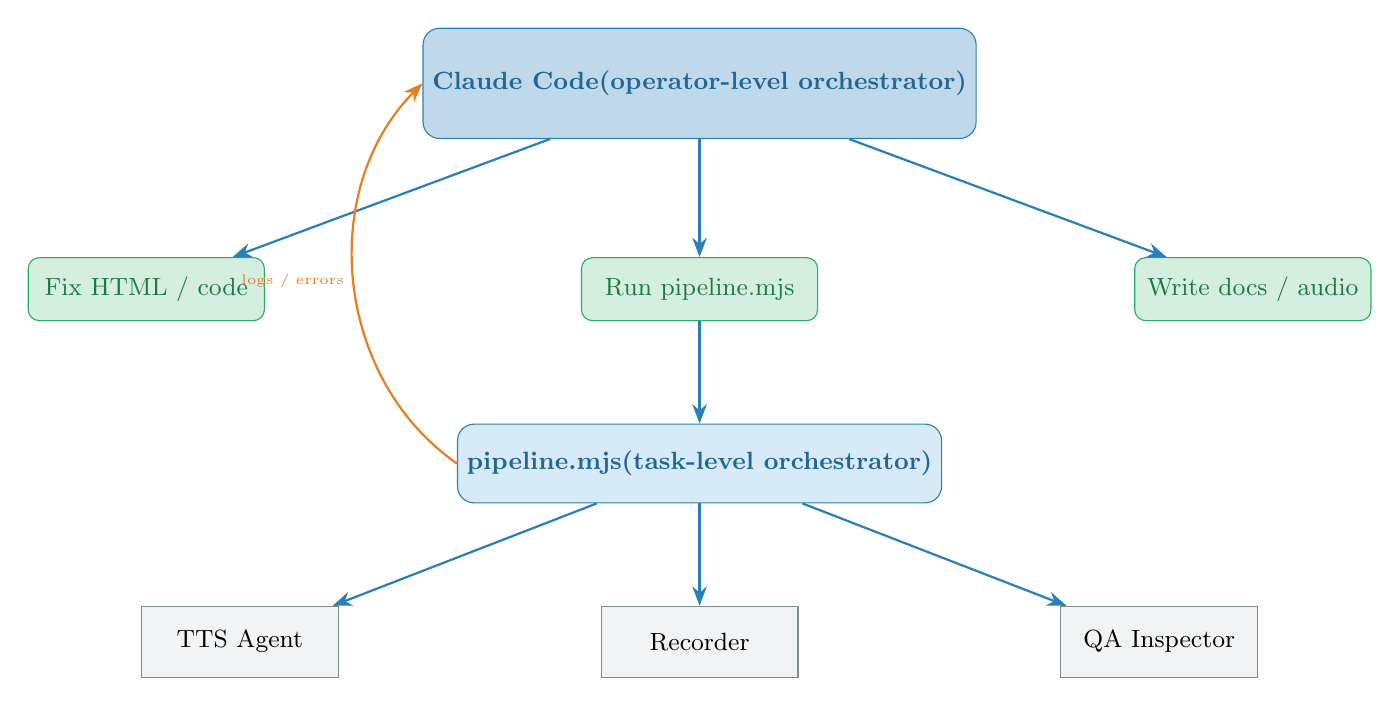
\begin{tikzpicture}
  \node[agent, fill=agentblue!30, draw=agentblue, minimum width=4cm,
        minimum height=1.4cm] (cc)
    {\textbf{Claude Code}\\{\small (operator-level orchestrator)}};

  \node[tool, below left=1.5cm and 2cm of cc, minimum width=3cm] (fix)
    {Fix HTML / code};
  \node[tool, below=1.5cm of cc, minimum width=3cm] (run)
    {Run pipeline.mjs};
  \node[tool, below right=1.5cm and 2cm of cc, minimum width=3cm] (docs)
    {Write docs / audio};

  \node[agent, below=1.3cm of run, minimum width=3.5cm] (pipe)
    {pipeline.mjs\\{\small (task-level orchestrator)}};

  \node[process, below left=1.3cm and 1.5cm of pipe, minimum width=2.5cm] (tts)
    {TTS Agent};
  \node[process, below=1.3cm of pipe, minimum width=2.5cm] (rec)
    {Recorder};
  \node[process, below right=1.3cm and 1.5cm of pipe, minimum width=2.5cm] (qa)
    {QA Inspector};

  \draw[arrowblue] (cc) -- (fix);
  \draw[arrowblue] (cc) -- (run);
  \draw[arrowblue] (cc) -- (docs);
  \draw[arrowblue] (run) -- (pipe);
  \draw[arrowblue] (pipe) -- (tts);
  \draw[arrowblue] (pipe) -- (rec);
  \draw[arrowblue] (pipe) -- (qa);

  \draw[arroworange, bend left=50] (pipe.west)
    to node[left, font=\tiny, color=agentorange]{logs / errors} (cc.west);
\end{tikzpicture}
\caption{Two-level orchestration: Claude Code (subscription, zero marginal cost)
         orchestrates pipeline.mjs which in turn orchestrates task-level agents
         (API calls).}
\end{figure}

\noindent\textbf{Key insight:} The expensive API calls (QA inspection, TTS) happen
inside \texttt{pipeline.mjs} using the OpenAI and Anthropic APIs. But the
\emph{meta-level} decisions --- what to build, how to fix bugs, what to monitor ---
are made by Claude Code at zero additional cost. Restructuring the system to move
more logic into Claude Code's orchestration layer and fewer decisions into
direct API calls would further reduce costs.

% =============================================================================
\section{Pipeline Implementation in Detail}
\label{sec:impl}
% =============================================================================

\subsection{Code Architecture}

The pipeline is implemented as a set of ES module (\texttt{.mjs}) files
orchestrated by \texttt{pipeline.mjs}. The directory structure is:

\begin{lstlisting}[language={},caption=Project structure]
Agentic_lecture_01/
  pipeline.mjs              # Main orchestrator
  sections.json             # 45-section configuration
  Asymptotic_Notation_Explorer.html  # Interactive tool
  agents/
    tts-agent.mjs           # OpenAI TTS wrapper + quality checks
    recorder.mjs            # Playwright screencast capture
    quality-inspector.mjs   # Vision QA via Claude API
    assembler.mjs           # FFmpeg video assembly
    navigator.mjs           # Browser navigation + cursor overlay
    section-planner.mjs     # LLM-based section script planning
    tool-qa.mjs             # HTML tool quality validation
    tool-evolver.mjs        # (disabled) LLM-driven HTML mutation
    video-qa.mjs            # Post-assembly video quality checks
    conversation-monitor.mjs # Human review integration
  utils/
    claude-agent.mjs        # Claude CLI subprocess wrapper
  docs/
    agentic_system_theory.tex   # This document
    make_audiobook.mjs          # Audiobook generator
  runs/
    run_XXXXX/              # One directory per pipeline run
      state.json            # Resumable state
      frames/               # PNG screenshots per section
      audio/                # MP3 files per section
      segments/             # Per-section .mp4 files
\end{lstlisting}

\subsection{The Orchestrator: \texttt{pipeline.mjs}}

\texttt{pipeline.mjs} is a single-file Node.js ESM script (~600 lines) that
drives the entire pipeline sequentially. Its key design characteristics are:

\begin{itemize}[leftmargin=2em]
  \item \textbf{No framework dependency} --- pure Node.js with npm packages only
        for Playwright, OpenAI SDK, and ffmpeg bindings
  \item \textbf{Explicit state machine} --- a \texttt{RunState} object is loaded
        or created at startup and saved after every section
  \item \textbf{CLI flags} for skipping stages:
        \texttt{--skip-planning}, \texttt{--skip-quality-loop},
        \texttt{--skip-tool-qa}, \texttt{--no-human-review}
  \item \textbf{Single browser instance} shared across all sections, restarted
        on crash detection
\end{itemize}

\begin{lstlisting}[language=JavaScript,caption=Core section loop in pipeline.mjs]
for (const section of sections) {
  if (state.completedSections.includes(section.id)) continue; // resume

  // 1. Generate TTS
  const { audioPath, duration } = await generateTTS(section.narration, ...);

  // 2. Switch tab + verify DOM
  await switchTabVerified(page, section.targetTab);

  // 3. Pre-select algorithm if needed
  if (section.algoSetup) await page.evaluate(section.algoSetup);

  // 4. Record screencast synchronised to audio
  const frames = await recordSectionLive(page, audioPath, duration);

  // 5. QA: DOM check overrides LLM vision for tab correctness
  const qa = await inspectQuality(frames[midFrame], section);
  qa.correct_tab = await verifyTabDOM(page, section.targetTab);

  // 6. Retry if tab wrong or content mismatch (NOT text_readable)
  if (!qa.correct_tab || !qa.content_matches) { retry; continue; }

  state.complete(section.id, { frames, audioPath, qa });
  await state.save();
}
\end{lstlisting}

\subsection{The Recorder: \texttt{recorder.mjs}}

The recorder uses Playwright's \texttt{page.screencast()} API to capture frames
at 5 fps during real-time audio playback. The key insight is that the recording
is \emph{wall-clock synchronised}: the screencast runs for exactly the audio
duration, producing a frame sequence that, when encoded at the correct frame
rate, has perfect lip-sync with the narration.

\begin{lstlisting}[language=JavaScript,caption=Live recording synchronised to audio duration]
export async function recordSectionLive(page, audioPath, duration) {
  const frames = [];
  const interval = 1000 / FPS;           // 200ms between frames
  const totalFrames = Math.ceil(duration * FPS);

  // GPU layout flush before starting
  await page.evaluate(() => document.body.getBoundingClientRect());
  await page.waitForTimeout(200);

  const startTime = Date.now();
  while (frames.length < totalFrames) {
    const screenshot = await page.screenshot({ type: 'png' });
    frames.push(screenshot);
    const elapsed = Date.now() - startTime;
    const nextCapture = frames.length * interval;
    const wait = Math.max(0, nextCapture - elapsed);
    if (wait > 0) await page.waitForTimeout(wait);
  }
  return frames;
}
\end{lstlisting}

\subsection{The QA Inspector: \texttt{quality-inspector.mjs}}

The QA inspector is a structured LLM call with a vision payload. A sample frame
(PNG) is base64-encoded and sent to \texttt{claude-sonnet-4-6} with a detailed
rubric prompt. The response is a JSON object matching a fixed schema:

\begin{lstlisting}[language=JavaScript,caption=QA inspector prompt structure]
const prompt = `
You are a quality inspector for lecture video frames.
Evaluate this screenshot against the following 6-point checklist:
1. correct_tab: Is the "${expectedTab}" tab active?
2. text_readable: Are chart axis labels and body text legible?
3. pointer_visible: Is the red cursor dot visible?
4. content_matches: Does the visual content match "${sectionDescription}"?
5. right_panel_active: Does the right panel show a chart or visualisation?
6. space_utilized: Does the content fill at least 60% of available space?

SCORING: correct_tab=false => score=0. content_matches=false => score=0.
Return JSON: { checklist: {...}, score: 0-100, issues: [...] }
`;
\end{lstlisting}

% =============================================================================
\section{Why Serving the HTML Over HTTP Solves the \texttt{file://} Problems}
\label{sec:http}
% =============================================================================

\subsection{The Root Problem: How Browsers Treat \texttt{file://} URLs}

When Playwright loads a page via a \texttt{file://} URL (e.g.\
\texttt{file:///Users/arash/.../Asymptotic\_Notation\_Explorer.html}),
the browser applies a fundamentally different set of rules than it does for
\texttt{http://} URLs. These differences caused three separate, compounding
bugs in the pipeline before the HTTP server was introduced.

\subsection{Problem 1: \texttt{waitUntil: 'networkidle'} Resolves Instantly}

Playwright's \texttt{page.goto()} accepts a \texttt{waitUntil} option that
controls when the navigation is considered complete. The \texttt{'networkidle'}
value means: \emph{wait until there have been no network requests for at least
500\,ms}.

\begin{lstlisting}[language=JavaScript,caption=The deceptive networkidle with file://]
// With file:// — resolves in <10ms (no network = always idle)
await page.goto('file:///path/to/tool.html', { waitUntil: 'networkidle' });
// ← code continues here immediately, before the page has rendered

// With http:// — resolves after real network activity settles
await page.goto('http://127.0.0.1:PORT/tool.html', { waitUntil: 'networkidle' });
// ← code continues only after all JS/CSS/font requests complete
\end{lstlisting}

\noindent\textbf{Why this matters:} The HTML tool loads Chart.js and executes
initialisation JavaScript that sets up the tab panels, renders charts, and applies
CSS classes. With \texttt{file://}, Playwright's navigation promise resolves
before any of this has happened, because there are no HTTP requests to wait for.
The subsequent \texttt{page.screenshot()} captures a partially-rendered or blank
page.

With an HTTP server, the browser makes real HTTP requests for the HTML document,
any referenced scripts or stylesheets, and fonts. The \texttt{networkidle}
condition correctly fires only after all these resources have loaded and the
JavaScript has had time to execute.

\begin{figure}[h]
\centering
\begin{tikzpicture}[x=0.9cm, y=0.8cm]
  % Axis
  \draw[thick,->,color=agentgray] (0,0) -- (12,0) node[right,font=\small]{time (ms)};

  % file:// timeline
  \node[font=\small\bfseries, color=agentred, left=0.1cm of {(0,2)}]
    {\texttt{file://}};
  \fill[agentblue!60]  (0,1.6) rectangle (0.3,2.4)
    node[above, font=\tiny, color=agentblue]{parse};
  \fill[agentred!60]   (0.3,1.6) rectangle (0.6,2.4)
    node[above right, font=\tiny, color=agentred]{\textbf{idle!}};
  \fill[agentgray!40]  (0.6,1.6) rectangle (3.5,2.4)
    node[midway, font=\tiny]{JS init (still running)};
  \draw[arrowred, thick] (0.6, 2.4) -- ++(0, 0.5)
    node[above, font=\tiny, color=agentred]{screenshot taken (blank)};

  % http:// timeline
  \node[font=\small\bfseries, color=agentgreen, left=0.1cm of {(0,0.5)}]
    {\texttt{http://}};
  \fill[agentblue!60]  (0,0.1) rectangle (0.3,0.9)
    node[above, font=\tiny, color=agentblue]{parse};
  \fill[agentgreen!50] (0.3,0.1) rectangle (1.2,0.9)
    node[midway, font=\tiny]{HTML req};
  \fill[agentgreen!50] (1.2,0.1) rectangle (2.4,0.9)
    node[midway, font=\tiny]{JS/CSS};
  \fill[agentblue!40]  (2.4,0.1) rectangle (3.5,0.9)
    node[midway, font=\tiny]{JS init};
  \fill[agentgreen!70] (3.5,0.1) rectangle (4.0,0.9)
    node[above right, font=\tiny, color=agentgreen!70!black]{\textbf{idle}};
  \draw[arrowgreen, thick] (4.0, 0.9) -- ++(0, 0.5)
    node[above, font=\tiny, color=agentgreen!70!black]{screenshot taken (rendered)};
\end{tikzpicture}
\caption{\texttt{file://} triggers \emph{networkidle} before JavaScript initialisation
completes. HTTP waits until all resource requests finish and the page is fully rendered.}
\end{figure}

\subsection{Problem 2: Page Reload Semantics Are Unreliable for \texttt{file://}}

Between recording sections, the pipeline reloads the page to reset interactive
state (sliders, selected algorithms, chart state). For \texttt{file://} URLs,
\texttt{page.reload()} behaves inconsistently across Chrome versions:

\begin{itemize}[leftmargin=2em]
  \item Some Chrome versions serve the page from the \textbf{disk cache} rather
        than re-reading the file from disk, meaning HTML edits (such as the
        \texttt{display:none} fix applied mid-run) are not picked up
  \item The \texttt{Cache-Control} header cannot be set for \texttt{file://}
        responses --- the browser decides caching behaviour unilaterally
  \item \texttt{waitUntil: 'networkidle'} on reload has the same instant-resolve
        problem as on initial load (Problem 1 above)
\end{itemize}

The HTTP server solves this by setting \texttt{Cache-Control: no-store} on
every response, guaranteeing that every reload fetches a fresh copy of the HTML
from disk:

\begin{lstlisting}[language=JavaScript,caption=Cache-Control header in the embedded HTTP server]
const server = createServer(async (req, res) => {
  const filePath = resolveFilePath(req.url, toolDir);
  res.writeHead(200, {
    'Content-Type': mimeTypes[ext] || 'text/plain',
    'Cache-Control': 'no-store'   // browser must re-fetch every time
  });
  createReadStream(filePath).pipe(res);
});
\end{lstlisting}

\noindent This also means that if the HTML tool is edited mid-run (e.g.\ to fix
a rendering bug), the very next section reload picks up the change with no
special handling required.

\subsection{Problem 3: Origin Restrictions Break JavaScript APIs}

The \texttt{file://} origin is treated as a \emph{null origin} by browsers.
This causes several Web APIs to silently fail or behave differently:

\begin{itemize}[leftmargin=2em]
  \item \textbf{Web Workers} cannot be spawned from \texttt{file://} pages in
        Chrome (used by some Chart.js rendering paths)
  \item \textbf{ES module imports} (\texttt{import}) are blocked on
        \texttt{file://} in Chrome without \texttt{--allow-file-access-from-files}
  \item \textbf{localStorage} and \textbf{sessionStorage} are inaccessible from
        \texttt{file://} null-origin contexts in strict mode
  \item \textbf{Fetch API} calls to relative URLs resolve incorrectly, as there
        is no base URL to resolve against
  \item \textbf{CORS preflight} checks always block cross-origin requests from
        a null origin, preventing the page from loading remote fonts or icons
\end{itemize}

Serving over \texttt{http://127.0.0.1} gives the page a proper origin
(\texttt{http://127.0.0.1:\{port\}}), resolving all of these restrictions.

\subsection{Problem 4: Query String Parameters Are Silently Ignored}

The original pipeline appended a cache-busting query parameter to force reloads:

\begin{lstlisting}[language=JavaScript,caption=Cache-busting hack (no longer needed)]
// Old workaround: append ?cachebust=<timestamp> to force reload
await page.goto(`file:///path/tool.html?cachebust=${Date.now()}`);
// Chrome ignores query strings entirely for file:// URLs
// This had zero effect — the cached version was served anyway
\end{lstlisting}

\noindent Chrome strips query parameters from \texttt{file://} URLs before
cache lookup, so \texttt{?cachebust=1774291347} and \texttt{?cachebust=1774291999}
resolve to the same cached file. The workaround \emph{appeared} to work in some
tests (coinciding with cache eviction) but was fundamentally inert.

With an HTTP server, query parameters are transmitted to the server and can be
acted upon (though with \texttt{Cache-Control: no-store} they are no longer
necessary).

\subsection{The HTTP Server Implementation}

The server is embedded directly in \texttt{pipeline.mjs} using Node.js's
built-in \texttt{http} module --- no external dependencies, no separate process:

\begin{lstlisting}[language=JavaScript,caption=Full embedded HTTP server (pipeline.mjs)]
import { createServer } from 'http';
import { createReadStream } from 'fs';
import { stat } from 'fs/promises';
import { join, basename, dirname } from 'path';

function startToolServer(toolPath) {
  const toolDir  = dirname(toolPath);
  const toolFile = basename(toolPath);

  return new Promise((resolve, reject) => {
    const server = createServer(async (req, res) => {
      // Strip query string and fragment from URL
      const urlPath  = req.url.split('?')[0].split('#')[0];

      // Map / and /toolFile to the HTML file; everything else is a sibling file
      const filePath = (urlPath === '/' || urlPath === `/${toolFile}`)
        ? toolPath
        : join(toolDir, urlPath.replace(/^\//, ''));

      const ext = filePath.split('.').pop().toLowerCase();
      const mimeTypes = {
        html: 'text/html', js: 'application/javascript',
        css: 'text/css',   json: 'application/json',
        png: 'image/png',  jpg: 'image/jpeg', svg: 'image/svg+xml'
      };

      try {
        await stat(filePath);            // throws if file doesn't exist
        res.writeHead(200, {
          'Content-Type':  mimeTypes[ext] || 'text/plain',
          'Cache-Control': 'no-store'    // always fresh
        });
        createReadStream(filePath).pipe(res);
      } catch {
        res.writeHead(404); res.end('Not found');
      }
    });

    // port 0 = OS assigns a free port automatically
    server.listen(0, '127.0.0.1', () => {
      const port = server.address().port;
      console.log(`  Tool server: http://127.0.0.1:${port}/${toolFile}`);
      resolve({ server, port, url: `http://127.0.0.1:${port}/${toolFile}` });
    });

    server.on('error', reject);
  });
}
\end{lstlisting}

\noindent Key design decisions:
\begin{itemize}[leftmargin=2em]
  \item \textbf{Port 0}: the OS assigns a random available port, avoiding
        conflicts with other services running on the machine
  \item \textbf{127.0.0.1}: binds to loopback only --- not accessible from the
        network, so no security exposure
  \item \textbf{Streaming response}: \texttt{createReadStream().pipe(res)} sends
        the file in chunks without loading it fully into memory --- important for
        large HTML files
  \item \textbf{Single server for all sections}: started once before Stage 3
        and closed once after Stage 5, avoiding the overhead of creating a new
        server per section
\end{itemize}

\subsection{Summary: \texttt{file://} vs \texttt{http://} for Playwright Automation}

\begin{table}[h]
\centering\small
\begin{tabular}{@{}p{4.5cm}p{4cm}p{4cm}@{}}
\toprule
\textbf{Behaviour} & \textbf{\texttt{file://}} & \textbf{\texttt{http://}} \\
\midrule
\texttt{waitUntil: 'networkidle'} &
  Resolves instantly (no network) &
  Resolves after real requests finish \\
\addlinespace
Reload semantics &
  May serve from disk cache; \texttt{Cache-Control} header ignored &
  Respects \texttt{Cache-Control: no-store}; always fetches fresh \\
\addlinespace
Query string cache-busting &
  Silently ignored by Chrome &
  Works as expected \\
\addlinespace
ES module imports &
  Blocked (null origin) &
  Allowed \\
\addlinespace
Web Workers &
  Blocked in Chrome &
  Allowed \\
\addlinespace
localStorage &
  Restricted (null origin) &
  Works normally \\
\addlinespace
Relative URL resolution &
  Fragile / broken &
  Correct base URL \\
\addlinespace
CORS / fetch to subresources &
  Blocked (null origin) &
  Works with proper headers \\
\bottomrule
\end{tabular}
\caption{Behavioural differences between \texttt{file://} and \texttt{http://}
in Playwright / Chrome automation contexts.}
\end{table}

% =============================================================================
\section{Framework Comparison: Custom Pipeline vs.\ LangGraph vs.\ n8n}
\label{sec:comparison}
% =============================================================================

\subsection{Overview}

The same agentic lecture production pipeline could, in principle, be built
with any of three approaches: (1) our custom Node.js implementation,
(2) LangGraph (a Python graph-based agent framework), or
(3) n8n (a visual no-code/low-code workflow automation platform).
Each embodies a different philosophy about how agent logic should be
expressed and executed.

\begin{table}[h]
\centering\small
\begin{tabular}{@{}lllll@{}}
\toprule
 & \textbf{Custom (ours)} & \textbf{LangGraph} & \textbf{n8n} \\
\midrule
Language       & JavaScript/Node.js & Python          & JSON / JS expressions \\
Paradigm       & Imperative code    & Graph of nodes  & Visual workflow \\
State          & \texttt{state.json} file & LangGraph State dict & Workflow execution context \\
LLM access     & Direct API calls   & LangChain LLMs  & HTTP Request nodes \\
Tool execution & Native JS + npm    & LangChain tools & Built-in nodes + HTTP \\
Branching      & \texttt{if/else} code & Conditional edges & If/Switch nodes \\
Retry logic    & Manual loop        & Retry nodes / edges & Error branch + retry node \\
Parallelism    & \texttt{Promise.all} & Parallel branches  & Split/merge nodes \\
Observability  & \texttt{console.log} & LangSmith tracing & n8n execution log \\
Hosting        & Local / any server & LangServe / cloud & n8n cloud / self-hosted \\
Learning curve & High (code)        & Medium (Python + graph) & Low (visual) \\
\bottomrule
\end{tabular}
\caption{Comparison of implementation approaches for the lecture production pipeline.}
\end{table}

\subsection{LangGraph}

LangGraph models an agent workflow as a \emph{directed graph} where nodes are
Python functions (or LLM calls) and edges carry state between them. Conditional
edges implement branching and retry loops.

\begin{lstlisting}[language=Python,caption=LangGraph sketch of the section recording loop]
from langgraph.graph import StateGraph, END
from typing import TypedDict

class PipelineState(TypedDict):
    section: dict
    audio_path: str
    frames: list
    qa_result: dict
    attempt: int

graph = StateGraph(PipelineState)

graph.add_node("tts",      generate_tts_node)
graph.add_node("switch_tab", switch_tab_node)
graph.add_node("record",   record_node)
graph.add_node("qa",       qa_inspect_node)

def should_retry(state):
    qa = state["qa_result"]
    if not qa["correct_tab"] or not qa["content_matches"]:
        if state["attempt"] < 2:
            return "record"   # retry edge
    return END

graph.add_edge("tts", "switch_tab")
graph.add_edge("switch_tab", "record")
graph.add_edge("record", "qa")
graph.add_conditional_edges("qa", should_retry)

app = graph.compile()
\end{lstlisting}

\textbf{What LangGraph adds} over our custom implementation:
\begin{itemize}[leftmargin=2em]
  \item \textbf{Built-in state checkpointing} via LangGraph's \texttt{MemorySaver}
        (our system replicates this manually with \texttt{state.json})
  \item \textbf{Visual graph inspection} --- the compiled graph can be rendered
        as a diagram for debugging
  \item \textbf{LangSmith tracing} --- every node invocation is automatically
        traced, logged, and inspectable in the LangSmith UI
  \item \textbf{Human-in-the-loop} via \texttt{interrupt\_before} / \texttt{interrupt\_after}
        node modifiers (we implement this manually with a CLI prompt)
  \item \textbf{Time travel} --- replay from any checkpoint for debugging
\end{itemize}

\textbf{What our implementation does better}:
\begin{itemize}[leftmargin=2em]
  \item \textbf{Playwright integration} is natural in Node.js (the Playwright
        library is JavaScript-native; the Python bindings are secondary)
  \item \textbf{FFmpeg integration} is simpler via \texttt{child\_process.execSync}
        than through Python subprocess wrappers
  \item \textbf{No framework overhead} --- no dependency on LangChain's
        abstractions, which add latency and version-incompatibility risks
  \item \textbf{Transparent logic} --- every decision is explicit in the code,
        not hidden inside a framework node
\end{itemize}

\subsection{n8n}

n8n is a visual workflow automation tool. Workflows are built by connecting
nodes in a canvas, with each node performing a specific action (HTTP request,
code execution, file operation, LLM call via built-in AI nodes).

\textbf{n8n equivalent of our pipeline} would look like:

\begin{enumerate}[leftmargin=2em]
  \item \textbf{Loop Over Items} node iterating over \texttt{sections.json}
  \item \textbf{HTTP Request} node calling OpenAI TTS API
  \item \textbf{Execute Command} node running a Playwright script (as a shell
        command, since n8n cannot control a browser natively)
  \item \textbf{HTTP Request} node calling Claude API with a base64 screenshot
  \item \textbf{IF} node checking \texttt{qa.correct\_tab \&\& qa.content\_matches}
  \item \textbf{Loop} back to step 3 if check fails (up to 2 retries)
  \item \textbf{Execute Command} node running FFmpeg for assembly
\end{enumerate}

\textbf{n8n advantages}:
\begin{itemize}[leftmargin=2em]
  \item \textbf{Zero coding} for the workflow structure --- business logic is
        visual and immediately understandable by non-engineers
  \item \textbf{Built-in credentials management} for API keys
  \item \textbf{Execution history} --- every workflow run is logged with
        input/output for every node
  \item \textbf{Scheduling, webhooks, triggers} --- easy to run on a cron,
        triggered by a file upload, or fired by a webhook
  \item \textbf{Self-hosted or cloud} with a web UI accessible from any device
        (addressing the user's remote monitoring need directly)
\end{itemize}

\textbf{n8n limitations for this pipeline}:
\begin{itemize}[leftmargin=2em]
  \item \textbf{No native browser control} --- Playwright must still be invoked
        as a shell command, making the DOM verification and tab switching logic
        opaque to n8n
  \item \textbf{Limited custom code} --- complex logic (the GPU flush, the
        5-attempt DOM retry loop) must live in \texttt{Code} nodes as JavaScript,
        essentially recreating our pipeline inside n8n boxes
  \item \textbf{File handling is awkward} --- passing large binary data (PNG
        frames, MP3 files) between nodes requires temporary files and path
        management
  \item \textbf{Stateful resumption} requires external storage (a database node)
        --- n8n's built-in state does not persist partial workflow runs
\end{itemize}

\subsection{What Is Common to All Three Approaches}

Regardless of framework, every implementation of this pipeline must handle the
same fundamental concerns:

\begin{enumerate}[leftmargin=2em]
  \item \textbf{External API calls} (OpenAI TTS, Anthropic QA) with
        authentication and error handling
  \item \textbf{Browser automation} for tab switching and screen capture
        (Playwright or Selenium in all cases)
  \item \textbf{State persistence} to support crash recovery and idempotent
        re-runs (file, database, or LangGraph checkpoint)
  \item \textbf{Retry logic} with a bounded maximum attempt count
  \item \textbf{Media processing} via FFmpeg for video assembly
  \item \textbf{Quality verification} using LLM vision after each recording
\end{enumerate}

The frameworks differ only in \emph{how} these concerns are expressed and
\emph{what} infrastructure they provide for observability, scheduling, and
human oversight.

% =============================================================================
\section{Claude Services and Components in Agentic Systems}
\label{sec:claude_services}
% =============================================================================

Anthropic offers several distinct products and APIs that serve different roles
in an agentic architecture. Understanding which component to use for which
purpose is essential for cost-effective, correct system design.

\begin{table}[h]
\centering\small
\begin{tabular}{@{}p{3cm}p{3.5cm}p{3cm}p{3.5cm}@{}}
\toprule
\textbf{Component} & \textbf{What it is} & \textbf{Billing} & \textbf{Best for} \\
\midrule
\textbf{Claude API} &
  REST API for text/vision inference. Models: Haiku 4.5, Sonnet 4.6, Opus 4.6 &
  Per input+output token &
  Automated pipelines, production systems \\
\addlinespace
\textbf{Claude Code} &
  CLI tool; agentic assistant with built-in tools (Bash, file I/O, web search) &
  Flat subscription (Max plan) &
  Development, debugging, meta-orchestration \\
\addlinespace
\textbf{Claude.ai} &
  Web/mobile chat interface &
  Flat subscription &
  Manual tasks, document review, ideation \\
\addlinespace
\textbf{Workspaces / Projects} &
  Persistent conversation context with file uploads &
  Included in subscription &
  Long-running collaborative tasks \\
\addlinespace
\textbf{MCP (Model Context Protocol)} &
  Standard protocol for connecting tools/data sources to Claude &
  N/A (infrastructure) &
  Extending Claude Code with external tools \\
\addlinespace
\textbf{Claude Agent SDK} &
  Python/JS SDK for building multi-agent systems with Claude &
  API tokens &
  Programmatic agent orchestration \\
\bottomrule
\end{tabular}
\caption{Anthropic products and their roles in agentic systems.}
\end{table}

\subsection{How Our Pipeline Uses Claude Services}

\begin{itemize}[leftmargin=2em]
  \item \textbf{Claude API (Sonnet 4.6)} --- used by \texttt{quality-inspector.mjs}
        for vision-based QA of recorded frames, and by \texttt{tool-qa.mjs} for
        validating the HTML tool. These are direct REST calls using the
        \texttt{@anthropic-ai/sdk} npm package.
  \item \textbf{Claude Code} --- the meta-orchestrator for the entire project.
        Every code change, bug fix, diagnosis, document creation, and pipeline
        restart in this project was performed by Claude Code running as an
        autonomous agent in the terminal.
  \item \textbf{Claude Code's built-in Agent tool} --- used to spawn specialised
        subagents (e.g., the Explore agent for codebase analysis, the Plan agent
        for architectural decisions) without incurring additional API costs.
  \item \textbf{Claude Code's Memory system} --- persistent Markdown files
        at \texttt{\textasciitilde/.claude/projects/.../memory/} store lessons
        learned (e.g., ``never use tool-evolver'', ``always skip-quality-loop''),
        ensuring that hard-won debugging insights persist across sessions.
\end{itemize}

\subsection{The MCP Ecosystem}

The \textbf{Model Context Protocol} (MCP) is an open standard that allows
Claude Code (and the Claude API) to connect to external data sources and tools
through a standardised interface. MCP servers expose \emph{resources} (files,
database records, API responses) and \emph{tools} (callable functions) to the
Claude model.

For the lecture pipeline, MCP could be used to:
\begin{itemize}[leftmargin=2em]
  \item Connect Claude Code to the Playwright browser via an MCP browser-control
        server (eliminating the need for \texttt{pipeline.mjs} entirely)
  \item Expose the \texttt{runs/} directory as an MCP resource, allowing Claude
        Code to query completed sections directly without reading \texttt{state.json}
  \item Integrate with n8n via its MCP node, creating a hybrid visual+agentic
        workflow
\end{itemize}

% =============================================================================
\section{LLM Portability: Replacing Claude with GPT-4o, Qwen, or Others}
\label{sec:portability}
% =============================================================================

\subsection{Which Parts Are LLM-Dependent?}

The pipeline has exactly two LLM-dependent components:

\begin{enumerate}[leftmargin=2em]
  \item \textbf{QA Inspector} (\texttt{quality-inspector.mjs}) --- requires a
        \emph{vision-capable} LLM that can analyse a screenshot and return a
        structured JSON response
  \item \textbf{Section Planner / Tool QA / Tool Fixer} --- requires a \emph{text}
        LLM with strong code-generation capability (for rewriting HTML or
        generating narration scripts)
\end{enumerate}

All other components (TTS, Playwright recording, FFmpeg assembly, HTTP server,
DOM verification) are \textbf{LLM-independent} and would remain identical
regardless of which language model is used.

\subsection{Replacing Claude with GPT-4o (OpenAI)}

GPT-4o is the most direct drop-in replacement. It supports vision, function
calling, and JSON-mode responses --- the exact capabilities our QA inspector
requires.

\begin{lstlisting}[language=JavaScript,caption=QA inspector with GPT-4o]
// Replace the Anthropic SDK call:
const response = await anthropic.messages.create({
  model: 'claude-sonnet-4-6',
  messages: [{ role: 'user', content: [
    { type: 'image', source: { type: 'base64', data: frameB64 }},
    { type: 'text', text: qaPrompt }
  ]}]
});

// With the OpenAI SDK call:
const response = await openai.chat.completions.create({
  model: 'gpt-4o',
  messages: [{ role: 'user', content: [
    { type: 'image_url',
      image_url: { url: `data:image/png;base64,${frameB64}` }},
    { type: 'text', text: qaPrompt }
  ]}],
  response_format: { type: 'json_object' }
});
\end{lstlisting}

The prompt itself needs no modification; the JSON output schema is identical.
The only change is the SDK call and the \texttt{Content} format.

\subsection{Replacing Claude with Qwen-VL (Alibaba)}

Qwen-VL is a strong open-source vision-language model available via the
DashScope API (Alibaba Cloud) or via Ollama for fully local inference. Using
Qwen-VL would make the QA inspection \textbf{completely free and private}:

\begin{lstlisting}[language=JavaScript,caption=QA inspector with Qwen-VL via Ollama]
// Run locally: ollama pull qwen2.5vl:7b
const response = await fetch('http://localhost:11434/api/generate', {
  method: 'POST',
  body: JSON.stringify({
    model: 'qwen2.5vl:7b',
    prompt: qaPrompt,
    images: [frameB64],  // base64 PNG
    stream: false,
    format: 'json'       // Ollama structured output
  })
});
const { response: text } = await response.json();
const qa = JSON.parse(text);
\end{lstlisting}

\textbf{Trade-offs with local models}:
\begin{itemize}[leftmargin=2em]
  \item \textbf{Inference speed}: a 7B model on an M5 Max GPU runs at
        $\sim$30--50 tokens/sec --- a QA call takes $\sim$10--20s vs
        $\sim$2--4s with the Claude API
  \item \textbf{Quality}: Qwen2.5-VL-7B is competitive on structured
        screenshot analysis but may be less consistent on ambiguous cases
        than Sonnet 4.6
  \item \textbf{Cost}: zero per-token cost after the initial model download
  \item \textbf{Privacy}: all inference stays on the local machine --- no
        lecture content is sent to external servers
\end{itemize}

\subsection{Replacing Claude with Gemini (Google)}

Gemini 2.0 Flash supports vision and structured JSON output via the Google
AI Studio API or Vertex AI. It has a generous free tier (1\,500 requests/day)
that could cover an entire pipeline run at no cost:

\begin{lstlisting}[language=JavaScript,caption=QA inspector with Gemini Flash]
import { GoogleGenerativeAI } from '@google/generative-ai';
const genai = new GoogleGenerativeAI(process.env.GEMINI_API_KEY);
const model = genai.getGenerativeModel({
  model: 'gemini-2.0-flash',
  generationConfig: { responseMimeType: 'application/json' }
});
const result = await model.generateContent([
  { inlineData: { mimeType: 'image/png', data: frameB64 }},
  qaPrompt
]);
const qa = JSON.parse(result.response.text());
\end{lstlisting}

\subsection{What Cannot Be Replaced: Claude Code as Meta-Orchestrator}

While the \emph{task-level} LLM (QA inspector, planner) can be swapped freely,
the \textbf{meta-level orchestrator} (Claude Code) is harder to replace. Claude
Code provides:

\begin{itemize}[leftmargin=2em]
  \item A persistent, tool-rich agentic environment with file I/O, Bash, and
        web access built in --- no scaffolding required
  \item The ability to \emph{read, understand, and modify its own pipeline code}
        --- a form of self-referential capability that general-purpose LLM APIs
        do not provide out of the box
  \item A memory system that persists engineering lessons across sessions
  \item A subscription model that makes the meta-level reasoning free
\end{itemize}

An equivalent could be built with OpenAI's Assistants API (with Code Interpreter
and file-search tools), Google's Gemini with function calling, or a local
\texttt{ollama} model paired with a custom agent loop. However, each would
require building the scaffolding that Claude Code provides natively.

\begin{figure}[h]
\centering
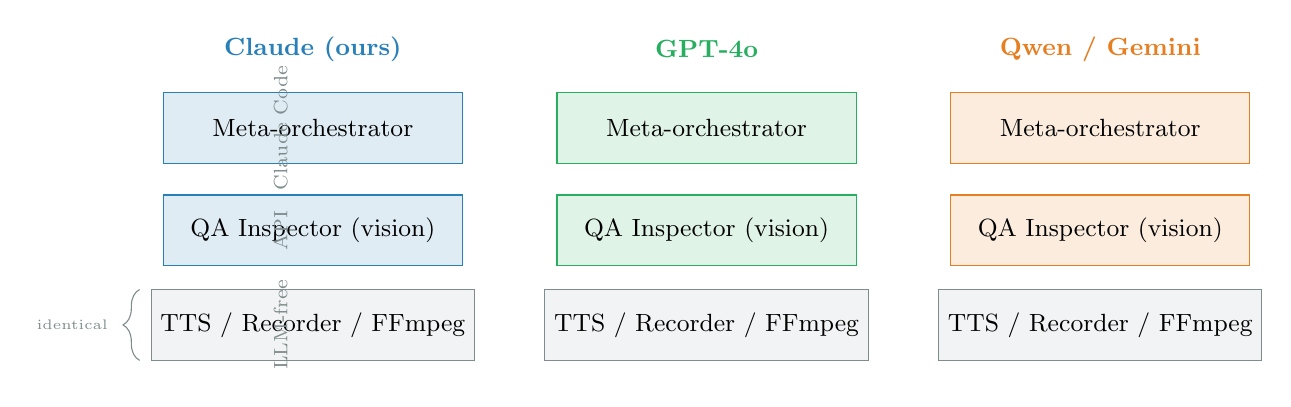
\begin{tikzpicture}
  % Header
  \node[font=\small\bfseries, color=agentblue] at (0, 4.5) {Claude (ours)};
  \node[font=\small\bfseries, color=agentgreen] at (5, 4.5) {GPT-4o};
  \node[font=\small\bfseries, color=agentorange] at (10, 4.5) {Qwen / Gemini};

  % Layers
  \foreach \x/\col in {0/agentblue, 5/agentgreen, 10/agentorange} {
    \node[process, draw=\col, fill=\col!15, minimum width=3.8cm,
          minimum height=0.9cm] at (\x, 3.5)
      {Meta-orchestrator};
    \node[process, draw=\col, fill=\col!15, minimum width=3.8cm,
          minimum height=0.9cm] at (\x, 2.2)
      {QA Inspector (vision)};
    \node[process, draw=agentgray, fill=lightgray, minimum width=3.8cm,
          minimum height=0.9cm] at (\x, 1.0)
      {TTS / Recorder / FFmpeg};
  }

  % Labels on left side
  \node[font=\small, color=agentgray, left=0.2cm of {(0,3.5)}]
    {\rotatebox{90}{\scriptsize Claude Code}};
  \node[font=\small, color=agentgray, left=0.2cm of {(0,2.2)}]
    {\rotatebox{90}{\scriptsize API}};
  \node[font=\small, color=agentgray, left=0.2cm of {(0,1.0)}]
    {\rotatebox{90}{\scriptsize LLM-free}};

  % Brace for LLM-free
  \draw[decorate, decoration={brace, amplitude=6pt}, color=agentgray]
    (-2.2, 0.55) -- (-2.2, 1.45)
    node[midway, left=8pt, font=\tiny, color=agentgray]{identical};
\end{tikzpicture}
\caption{The bottom layer (TTS, Playwright, FFmpeg) is identical across all LLM
choices. Only the top two layers change.}
\end{figure}

% =============================================================================
\begin{thebibliography}{9}
\bibitem{yao2023react}
  S.~Yao et al.,
  \textit{ReAct: Synergizing Reasoning and Acting in Language Models},
  ICLR 2023.

\bibitem{russell1995}
  S.~Russell and P.~Norvig,
  \textit{Artificial Intelligence: A Modern Approach},
  Prentice Hall, 1995.

\bibitem{shinn2023reflexion}
  N.~Shinn et al.,
  \textit{Reflexion: Language Agents with Verbal Reinforcement Learning},
  NeurIPS 2023.

\bibitem{wang2023planandsolve}
  L.~Wang et al.,
  \textit{Plan-and-Solve Prompting: Improving Zero-Shot Chain-of-Thought Reasoning},
  ACL 2023.

\bibitem{anthropic2024claude}
  Anthropic,
  \textit{Claude Technical Report},
  2024.
\end{thebibliography}

\end{document}
